%
% Exemplo LaTeX de monografia UNISINOS
%
% Elaborado com base nas orientações dadas no documento
% ``GUIA PARA ELABORAÇÃO DE TRABALHOS ACADÊMICOS''
% disponível no site da biblioteca da Unisinos.
% http://www.unisinos.br/biblioteca
%
% Os elementos textuais abaixo são apresentados na ordem em que devem
% aparecer no documento.  Repare que nem todos são obrigatórios - isso
% é devidamente indicado em cada caso.
%
% Comentários abaixo colocados entre aspas (`` '') foram
% extraídos diretamente do documento da biblioteca.
%
% Este documento é de domínio público.
%



%=======================================================================
% Declarações iniciais identificando a classe de documento e
% selecionando alguns pacotes adicionais.
%
% As opções disponíveis (separe-as com vírgulas, sem espaço) são:
% - twoside: Formata o documento para impressão frente-e-verso
%   (o default é somente-frente)
% - english,brazilian,french,german,etc.: idiomas usados no documento.
%   Deve ser colocado por último o idioma principal.
%=======================================================================
\documentclass[oneside,english,brazilian]{UNISINOSmonografia}
\usepackage[utf8]{inputenc} % charset do texto (utf8, latin1, etc.)
\usepackage[T1]{fontenc} % encoding da fonte (afeta a sep. de sílabas)
\usepackage{graphicx} % comandos para gráficos e inclusão de figuras
\usepackage{bibentry} % para inserir refs. bib. no meio do texto
\usepackage{float}
\usepackage{amsmath,amssymb}
\usepackage{booktabs}
\usepackage{multirow}
\usepackage{subcaption}

%=======================================================================
% Escolha do sistema para geração de referências bibliográficas.
%
% O default é usar o estilo unisinos.bst.  Comente a definição abaixo
% e descomente a linha seguinte para usar o estilo do ABNTeX (é
% necessário ter esse pacote instalado).
%
% A vantagem do unisinos.bst é que ele permite o uso de um arquivo .bib
% seguindo as orientações tradicionais do BibTeX (veja essas orientações
% em http://ctan.tug.org/tex-archive/biblio/bibtex/contrib/doc/btxdoc.pdf).
% Entretanto, o estilo não suporta algumas citações mais exóticas como
% apud.  Para isso, use o ABNTeX, mas esteja ciente de que muitas de
% suas referências serão incompatíveis com os estilos tradicionais do
% BibTeX como plain, alpha, ieeetr, entre outros.
%=======================================================================
\usepackage[alf]{abntex2cite}
%\usepackage[alf]{abntcite}

%=======================================================================
% Dados gerais sobre o trabalho.
%=======================================================================
\autor{Murakami}{Lucas Kaito}
\titulo{Benchmarking de Arquiteturas MobileNet para Detecção de Lesões Dermatológicas.}
%\subtitulo{}
\orientador[Dr.]{Moreira de Oliveira}{Flavio}
%\coorientador[Prof.~Dr.]{Lamport}{Leslie}

\unidade{Unidade Acadêmica de Graduação}
\curso{Curso de Bacharelado em Ciência da Computação}
\natureza{%
Monografia apresentada como requisito parcial para obtenção do título de Bacharel em Ciência da Computação, pelo Curso de Ciência da Computação da Universidade do Vale do Rio dos Sinos (UNISINOS)
}
\local{Porto Alegre}
\ano{2026}

% dados da ficha catalográfica
% (obrigatória somente para dissertações e teses)
%\cip{Dissertação (mestrado)}{004.732}
%\bibliotecario{Bibliotecária responsável: Fulana da Silva}{12/3456}

% cada palavra-chave deve ser fornecida duas vezes, uma em português e
% outra no idioma estrangeiro (na verdade, em tantos idiomas quantos se
% desejar).
\palavrachave{brazilian}{Câncer de pele}
\palavrachave{brazilian}{Computação de Borda}
\palavrachave{brazilian}{MobileNet}
\palavrachave{brazilian}{Dataset Shift}
\palavrachave{brazilian}{Inteligência Artificial}

\palavrachave{english}{Skin Cancer}
\palavrachave{english}{Edge Computing}
\palavrachave{english}{MobileNet}
\palavrachave{english}{Dataset Shift}
\palavrachave{english}{Artificial Intelligence}

%=======================================================================
% Início do documento.
%=======================================================================
\raggedbottom
\begin{document}
\capa
\folhaderosto
%\folhadeaprovacao % não deve ser incluída nos TCCs

%=======================================================================
% Dedicatória (opcional).
%
% O texto é normalmente colocado na parte de baixo da página, alinhado
% à direita.  Mas a formatação é basicamente livre.  Só não se escreve
% a palavra 'dedicatória'.
%=======================================================================
% \begin{dedicatoria}
% Aos nossos pais.\\[4ex] % quebra a linha dando um espaçamento maior
% \begin{itshape} % faz o texto ficar em itálico
% If I have seen farther than others,\\
% it is because I stood on the shoulders of giants.\\
% \end{itshape}
% --- \textsc{Sir Isaac Newton} % \textsc é o "small caps"
% \end{dedicatoria}

%=======================================================================
% Agradecimentos (opcional).
%=======================================================================
% \begin{agradecimentos}
% Obrigado!
% \end{agradecimentos}

%=======================================================================
% Epígrafe (opcional).
%
% ``[...] o autor apresenta uma citação, seguida de indicação de autoria,
% relacionada com a matéria tratada no corpo do trabalho. Podem, também,
% constar epígrafes nas folhas de aberturas das seções primárias.''
%=======================================================================
% \begin{epigrafe}
% ``\textit{Ninguém abre um livro sem que aprenda alguma coisa}''.\\
% (Anônimo)
% \end{epigrafe}

%=======================================================================
% Resumo em Português.
%
% A recomendação é para 150 a 500 palavras.
%=======================================================================
\begin{abstract}
O câncer de pele é o tumor de maior incidência no Brasil, e a detecção precoce do melanoma é crítica para reduzir a letalidade. Embora Redes Neurais Convolucionais (CNNs) alcancem alto desempenho em bases dermatoscópicas laboratoriais, sofrem degradação severa ao lidar com imagens clínicas de celulares em cenários reais (\textit{Dataset Shift}). Para viabilizar a triagem descentralizada, arquiteturas leves projetadas para computação de borda (\textit{edge computing}) tornam-se essenciais. Este trabalho realiza um \textit{benchmarking} técnico entre as cinco gerações da arquitetura MobileNet (V1 a V5), analisando o \textit{trade-off} entre complexidade estrutural (número de parâmetros) e resiliência diagnóstica na transição de domínio. Os modelos foram treinados por transferência de aprendizado em dois estágios no HAM10000, com particionamento estrito por lesão, amostragem balanceada, \textit{Focal Loss}, \textit{Mixup} e otimizador AdamW. A calibração de probabilidades (\textit{Temperature Scaling}) e os limiares operacionais (\textit{policy sens90}) foram ajustados na validação interna, e a generalização foi avaliada de forma cega no conjunto clínico PAD-UFES-20 (fotos de \textit{smartphones}). O desempenho foi avaliado através de três sementes pelas métricas de AUC-ROC, Sensibilidade (\textit{Recall}) de melanoma e malignidade conjunta, e Erro de Calibração Esperado (ECE). Os resultados evidenciaram um claro \textit{trade-off}: a MobileNetV5 atingiu a maior discriminação média (AUC de 0,765 no PAD), porém à custa de 294,1 milhões de parâmetros; entre os modelos genuinamente compactos, a MobileNetV4 (8,4M) apresentou o melhor compromisso de discriminação externa (AUC de 0,730 e menor ECE), enquanto a MobileNetV3 (4,2M) obteve a maior sensibilidade de triagem maligna (0,788). Contudo, o \textit{dataset shift} provocou quedas generalizadas de sensibilidade nos limiares transferidos em todas as versões. Conclui-se que não há um vencedor absoluto e que o ganho diagnóstico de modelos maiores deve ser pesado contra o custo computacional para triagem móvel, exigindo validação no domínio clínico alvo antes de qualquer implantação prática.
\end{abstract}

%=======================================================================
% Resumo em língua estrangeira (obrigatório somente para teses e
% dissertações).
%
% O idioma usado aqui deve necessariamente aparecer nos parâmetros do
% \documentclass, no início do documento.
%=======================================================================
\begin{otherlanguage}{english}
\begin{abstract}
Skin cancer is the most prevalent malignancy in Brazil, and early melanoma detection is critical to reducing mortality. Although Convolutional Neural Networks (CNNs) achieve high performance on curated dermoscopic benchmarks, they suffer severe degradation when applied to clinical smartphone imagery under real-world conditions (Dataset Shift). To enable decentralized screening, lightweight architectures designed for edge computing are essential. This work conducts a technical benchmark across the five evolutionary generations of the MobileNet architecture (V1 to V5), analyzing the trade-off between structural complexity (parameter count) and diagnostic resilience under domain shift. Models were trained via two-stage transfer learning on HAM10000 with lesion-grouped partitioning, balanced sampling, Focal Loss, Mixup, and the AdamW optimizer. Probability calibration (Temperature Scaling) and operating thresholds (sens90 policy) were tuned on internal validation, and generalization was blindly evaluated on the clinical PAD-UFES-20 dataset (uncontrolled smartphone photos). Evaluated across three random seeds via AUC-ROC, melanoma and joint malignancy Sensitivity (Recall), and Expected Calibration Error (ECE), the results demonstrate a clear trade-off: MobileNetV5 achieved the highest discrimination (PAD MEL AUC 0.765), but at the expense of 294.1M parameters; among compact models, MobileNetV4 (8.4M) delivered the strongest external discrimination trade-off (AUC 0.730, lowest ECE), while MobileNetV3 (4.2M) yielded the highest joint malignant screening recall (0.788). However, domain shift induced substantial sensitivity drops across all architectures when transferring operating thresholds. We conclude that no architecture universally dominates and that diagnostic gains in larger models must be weighed against computational cost for edge deployment, requiring target-domain threshold calibration prior to clinical adoption.
\end{abstract}
\end{otherlanguage}

%=======================================================================
% Lista de Figuras (opcional).
%=======================================================================
\listoffigures

%=======================================================================
% Lista de Tabelas (opcional).
%=======================================================================
\listoftables

%=======================================================================
% Lista de Abreviaturas (opcional).
%
% Deve ser passada como parâmetro a maior das abreviaturas utilizadas.
%=======================================================================
\begin{listadeabreviaturas}{app.}
\item[app.] aplicativo
\item[ex.] exemplo
\item[etc.] et cetera
\item[vs.] versus
\end{listadeabreviaturas}

%=======================================================================
% Lista de Siglas (opcional).
%
% Deve ser passada como parâmetro a maior das siglas utilizadas.
%=======================================================================
\begin{listadesiglas}{AUC-ROC}
\item[ABNT] Associação Brasileira de Normas Técnicas
\item[ACK] Queratose Actínica e Doença de Bowen (abreviação alternativa)
\item[AKIEC] Queratose Actínica e Doença de Bowen
\item[AUC-ROC] Área sob a Curva de Característica de Operação do Receptor (\textit{Area Under the Receiver Operating Characteristic Curve})
\item[BCC] Carcinoma Basocelular (\textit{Basal Cell Carcinoma})
\item[BKL] Queratose Seborreica
\item[CNN] Rede Neural Convolucional (\textit{Convolutional Neural Network})
\item[CPU] Unidade Central de Processamento (\textit{Central Processing Unit})
\item[DF] Dermatofibroma
\item[DSP] Processador de Sinal Digital (\textit{Digital Signal Processor})
\item[FLOPs] Operações de Ponto Flutuante (\textit{Floating Point Operations})
\item[FP32] Ponto Flutuante de 32 bits (\textit{32-bit Floating Point})
\item[GPU] Unidade de Processamento Gráfico (\textit{Graphics Processing Unit})
\item[IA] Inteligência Artificial
\item[INCA] Instituto Nacional de Câncer
\item[INT8] Inteiro de 8 bits (\textit{8-bit Integer})
\item[LLM] Modelo de Linguagem Grande (\textit{Large Language Model})
\item[MEL] Melanoma
\item[MQA] Atenção de Múltiplas Consultas Móvel (\textit{Mobile Multi-Query Attention})
\item[NAS] Busca de Arquitetura de Rede (\textit{Network Architecture Search})
\item[NEV] Nevos Melanocíticos (abreviação alternativa)
\item[NPU] Unidade de Processamento Neural (\textit{Neural Processing Unit})
\item[NV] Nevos Melanocíticos
\item[PTQ] Quantização Pós-Treinamento (\textit{Post-Training Quantization})
\item[RAM] Memória de Acesso Aleatório (\textit{Random Access Memory})
\item[SCC] Carcinoma Espinocelular (\textit{Squamous Cell Carcinoma})
\item[SE] Aperto-e-Excitação (\textit{Squeeze-and-Excitation})
\item[SEK] Queratose Seborreica (abreviação alternativa)
\item[TCC] Trabalho de Conclusão de Curso
\item[UIB] Bloco de Gargalo Invertido Universal (\textit{Universal Inverted Bottleneck})
\item[VASC] Lesões Vasculares
\end{listadesiglas}

%=======================================================================
% Lista de Símbolos (opcional).
%
% Deve ser passado o maior (mais largo) dos símbolos utilizados.
%=======================================================================
\begin{listadesimbolos}{$\tau_{\text{prior}}$}
\item[$\alpha$] Multiplicador de largura arquitetural (\textit{width multiplier})
\item[$\alpha_t$] Fator de ponderação de classe da \textit{Focal Loss}
\item[$\alpha_k^c$] Coeficiente de importância de ativação espacial do Grad-CAM
\item[$\gamma$] Fator de modulação de foco da \textit{Focal Loss} ($\gamma = 2{,}0$)
\item[$\lambda$] Coeficiente estocástico de combinação linear do \textit{Mixup}
\item[$\rho$] Multiplicador de resolução (\textit{resolution multiplier})
\item[$\tau^*$] Limiar de decisão contínuo sintonizado para triagem (política \texttt{sens90})
\item[$\tau_{\text{prior}}$] Coeficiente de escala para ajuste de logits por probabilidade a priori (\textit{prior correction})
\item[$T^*$] Escalar homotético ótimo de calibração de temperatura (\textit{Temperature Scaling})
\item[\%] Porcentagem
\item[$D_F$] Dimensão espacial do mapa de características (\textit{Feature map size})
\item[$D_K$] Dimensão do kernel convolucional espacial (\textit{Spatial kernel size})
\item[$M$] Número de canais de entrada (\textit{Input channels})
\item[$N$] Número de canais de saída ou tamanho amostral (\textit{Output channels})
\end{listadesimbolos}

%=======================================================================
% Sumário
%=======================================================================
\tableofcontents

%=======================================================================
% Introdução
%=======================================================================
\chapter{Introdução}

O câncer de pele é o tumor de maior incidência no Brasil, constituindo um desafio crítico para a saúde pública e para o sistema previdenciário. Segundo o Instituto Nacional do Câncer \cite{inca2026estimativa}, estima-se a ocorrência de aproximadamente 272.640 novos casos anuais para o triênio 2026-2028. A detecção precoce é o fator determinante para a redução da letalidade, especialmente nos casos de melanoma. Contudo, a escassez de especialistas em regiões remotas e a sobrecarga de atendimentos nos centros urbanos criam barreiras logísticas que dificultam o diagnóstico em tempo hábil.

Diante da necessidade de descentralização diagnóstica, a aplicação de Inteligência Artificial (IA) em dispositivos móveis apresenta-se como uma ferramenta de triagem automatizada promissora. O potencial das Redes Neurais Convolucionais (CNNs) na dermatologia foi validado de forma pioneira por \citeonline{esteva2017dermatologist}, que demonstraram que modelos de Aprendizado Profundo podem atingir níveis de classificação de câncer de pele comparáveis aos de dermatologistas certificados. Apesar dessas acurácias superiores a 95\% em laboratório, a literatura mais recente evidencia uma queda abrupta de desempenho no ambiente clínico real \cite{wolf2025deep}. A esmagadora maioria das arquiteturas é otimizada sobre bancos de dados dermatoscópicos perfeitamente curados e falha ao processar imagens ruidosas capturadas por câmeras comuns. Há, portanto, a necessidade técnica de validar modelos que suportem essa quebra de domínio (\textit{Dataset Shift}) sem exceder as limitações de \textit{hardware} dos celulares populares.

Este trabalho propõe um \textit{benchmarking} entre as gerações da arquitetura MobileNet (V1, V2, V3, V4 e V5), visando mitigar a lacuna entre a pesquisa acadêmica e a eficácia prática. A família MobileNet foi selecionada devido à sua base em Convoluções Separáveis em Profundidade, técnica projetada especificamente para viabilizar a inferência nativa em dispositivos de baixo poder computacional (\textit{edge computing}) \cite{howard2017mobilenets_google}. Para atestar a capacidade de generalização do algoritmo, o treinamento será conduzido na base de dados padronizada HAM10000, enquanto a validação ocorrerá de forma cega no \textit{dataset} brasileiro PAD-UFES-20 \cite{pacheco2020pad}, composto unicamente por imagens não controladas retiradas de \textit{smartphones}.

Ao longo deste estudo, busca-se quantificar o \textit{trade-off} entre a complexidade estrutural das redes (avaliada pela contagem de parâmetros e requisitos arquiteturais para computação de borda) e a resiliência diagnóstica frente à quebra de domínio. Devido ao desbalanceamento estatístico severo inerente à prática clínica ambulatorial, o desempenho não será pautado pela Acurácia Global, mas fundamentado pela Sensibilidade (\textit{Recall}) e pela métrica AUC-ROC, focando estritamente na minimização de Falsos Negativos. Os resultados esperados fornecerão evidências empíricas sobre qual geração arquitetural entrega melhores resultados para operar como tecnologia de triagem em larga escala no ecossistema de saúde brasileiro.

\section{Tema}
O tema desta pesquisa insere-se na área de Visão Computacional aplicada à saúde, com foco na utilização de Redes Neurais Convolucionais para a triagem e o diagnóstico assistido de lesões dermatológicas através de dispositivos móveis (\textit{edge computing}).

\section{Delimitação do Tema}
O escopo do estudo restringe-se ao \textit{benchmarking} quantitativo rigoroso das gerações V1 a V5 da arquitetura MobileNet. A avaliação foca na detecção de lesões malignas, com ênfase no melanoma e na triagem conjunta de malignidade, contrapondo o treinamento em imagens dermatoscópicas padronizadas (HAM10000) à inferência em imagens clínicas não controladas capturadas por \textit{smartphones} (PAD-UFES-20). A análise computacional concentra-se na caracterização da complexidade estrutural de parâmetros e requisitos de processamento para a borda e na avaliação de métricas clínicas frente ao desbalanceamento e quebra de domínio (Sensibilidade, AUC-ROC e Calibração ECE), delimitando a quantização física e o desenvolvimento de software aplicativo como etapas de trabalhos futuros.

\section{Problema}
Modelos de aprendizado profundo apresentam alta eficácia em bases de dados laboratoriais curadas, mas sofrem degradação severa de desempenho ao processar imagens ruidosas em cenários reais (\textit{Dataset Shift}). Diante desta lacuna, a questão central que guia esta pesquisa é: {Qual geração da arquitetura MobileNet apresenta o melhor equilíbrio (\textit{trade-off}) entre eficiência computacional em \textit{smartphones} populares e resiliência diagnóstica na triagem de melanoma frente ao ruído visual e desbalanceamento de classes inerentes ao cenário clínico brasileiro?}

\section{Objetivos}

O objetivo geral deste trabalho é realizar um \textit{benchmarking} rigoroso das gerações da arquitetura MobileNet (V1, V2, V3, V4 e V5), analisando o \textit{trade-off} entre a eficiência de processamento em hardware móvel e a capacidade de generalização diagnóstica em cenários clínicos reais.

\subsection{Objetivos Específicos}
Para o alcance do objetivo geral, definem-se os seguintes objetivos específicos:

\begin{itemize}
    \item Treinar e otimizar os modelos MobileNet utilizando dados controlados (HAM10000) e transferir a validação para dados do mundo real (PAD-UFES-20);
    \item Avaliar a robustez diagnóstica das arquiteturas perante o desbalanceamento severo de classes, utilizando a Sensibilidade (\textit{Recall}) e limiares operacionais clínicos como métricas primárias para minimizar Falsos Negativos;
    \item Mensurar a capacidade de separação de classes dos modelos através da métrica de Área sob a Curva ROC (AUC-ROC) e a confiabilidade preditiva via Erro de Calibração Esperado (ECE);
    \item Caracterizar e comparar a complexidade estrutural de cada geração arquitetural por meio da contagem de parâmetros e requisitos de processamento, mapeando os compromissos técnicos e a prontidão dos modelos para futura quantização e embarcação em aplicativos móveis.
\end{itemize}

\section{Justificativa}
A alta incidência de câncer de pele no Brasil e a concentração de especialistas em grandes centros urbanos exigem soluções tecnológicas descentralizadas para a triagem primária. Embora a literatura reporte índices de acurácia próximos a 98\% utilizando CNNs densas, a dependência de processamento em nuvem introduz gargalos de infraestrutura, latência e privacidade. A execução nativa no dispositivo (\textit{on-device}) resolve estas barreiras, mas impõe restrições severas de processamento e memória. 

A escolha por investigar as arquiteturas MobileNet justifica-se pela sua engenharia baseada em Convoluções Separáveis em Profundidade, concebida para hardware limitado. O \textit{benchmarking} direto no \textit{dataset} brasileiro PAD-UFES-20 é essencial porque sistemas de triagem médica não podem ser fundamentados em métricas infladas por imagens de laboratório (HAM10000). Identificar qual versão da MobileNet consegue manter um alto nível de Sensibilidade, garantindo que melanomas reais não sejam ignorados (Falsos Negativos) por distorções da câmera do celular, é um passo fundamental para atestar a segurança e a viabilidade da Inteligência Artificial como instrumento de saúde pública em escala nacional.

%=======================================================================
% Fundamentação Teórica
%=======================================================================

\chapter{Fundamentação Teórica}
Este capítulo estabelece a base conceitual fundamental para a compreensão desta pesquisa. A fundamentação é estruturada a partir do contexto médico e estatístico, abordando inicialmente a classificação clínica do câncer de pele e as patologias presentes nos \textit{datasets} dermatológicos. 

Em seguida, explora-se o escopo computacional da Inteligência Artificial, detalhando o funcionamento das Redes Neurais Convolucionais (CNNs) para a extração de características visuais e a evolução da arquitetura MobileNet projetada especificamente para a computação de borda (\textit{edge computing}). Na sequência, formaliza-se a teoria estatística da Mudança de Domínio (\textit{Dataset Shift}), conceituando \textit{Covariate Shift} e \textit{Prior Probability Shift}. Por fim, consolidam-se as métricas de avaliação diagnóstica e os \textit{trade-offs} computacionais essenciais para viabilizar a execução nativa e eficiente em dispositivos móveis.

\section{Câncer de Pele e a Classificação dos Datasets}

O câncer de pele caracteriza-se pelo crescimento anormal e descontrolado das células que compõem as camadas da pele. Clinicamente, o escopo diagnóstico vai muito além de uma divisão binária (doente ou saudável). Para que uma Rede Neural Convolucional seja eficaz, ela deve ser treinada para distinguir o melanoma de várias outras lesões que se assemelham visualmente a ele.

Dessa forma, os \textit{datasets} adotados nesta pesquisa (HAM10000 e PAD-UFES-20) abrangem o espectro das lesões de pele mais comuns na prática clínica ambulatorial. Elas dividem-se em dois grandes grupos:

\subsection{Lesões Malignas (Câncer)}
Este grupo engloba as patologias que apresentam crescimento destrutivo e potencial de letalidade.
\begin{itemize}
    \item \textbf{Melanoma (MEL):} É o tipo mais agressivo de câncer de pele, originado nos melanócitos (células produtoras de pigmento). Embora represente uma porcentagem menor dos casos totais, possui um alto risco de metástase, o processo no qual as células cancerígenas viajam pela corrente sanguínea ou sistema linfático para órgãos vitais. Seu diagnóstico precoce é o alvo principal (classe positiva) de sistemas de triagem.
    \item \textbf{Carcinoma Basocelular (BCC):} É a neoplasia maligna mais comum na população brasileira devido à exposição solar crônica. Possui crescimento muito lento e baixo risco de metástase, mas pode causar destruição tecidual profunda localmente.
    \item \textbf{Carcinoma Espinocelular (SCC):} O segundo tipo de câncer de pele não melanoma mais incidente. É mais agressivo que o basocelular e possui capacidade metastática se negligenciado.
\end{itemize}

\subsection{Lesões Pré-Malignas e Benignas}
Este grupo engloba neoplasias benignas e lesões pré-malignas precursoras que atuam como diagnósticos diferenciais ou alvos de triagem preventiva.
\begin{itemize}
    \item \textbf{Nevos Melanocíticos (NV / NEV):} São tumores benignos derivados dos melanócitos, popularmente conhecidos como "pintas" ou "sinais".
    \item \textbf{Queratose Actínica e Doença de Bowen (AKIEC / ACK):} São lesões pré-malignas causadas por dano solar severo. São consideradas o passo inicial antes do desenvolvimento de um Carcinoma Espinocelular, exigindo acompanhamento médico. Por sua progressão direta para o SCC e sobreposição visual em fotografia clínica, é incorporada ao grupo de triagem prioritária conjunta neste estudo.
    \item \textbf{Queratose Seborreica (BKL / SEK):} Tumores cutâneos benignos extremamente comuns em adultos. Geralmente, representam um desafio de Visão Computacional, pois frequentemente simulam a aparência do melanoma, confundindo o diagnóstico.
    \item \textbf{Dermatofibroma (DF):} Uma lesão benigna profunda constituída por fibroblastos.
    \item \textbf{Lesões Vasculares (VASC):} Englobam angiomas e angioceratomas. São pápulas ou nódulos benignos formados por vasos sanguíneos dilatados.
\end{itemize}

\section{Inteligência Artificial e Redes Neurais Convolucionais}
Entre outras aplicações, a Inteligência Artificial (IA) no contexto médico refere-se à capacidade de sistemas computacionais processarem grandes volumes de dados para identificar padrões diagnósticos. Este trabalho utiliza o Deep Learning (Aprendizado Profundo), especificamente as Redes Neurais Convolucionais (CNNs), cuja organização estrutural básica está representada na Figura~\ref{fig:cnn_architecture}.

\begin{figure}[H]
    \caption{Exemplificação de arquitetura CNN.}
    \label{fig:cnn_architecture}
    \centering
    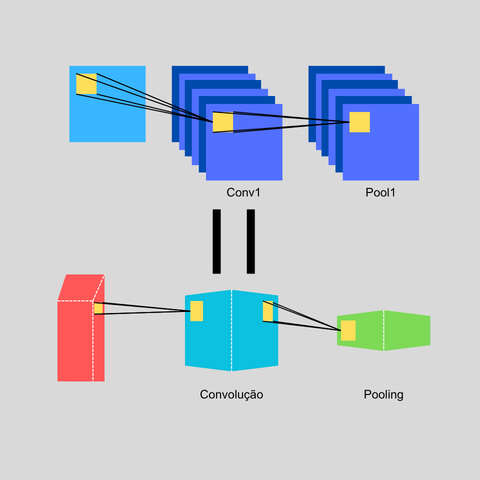
\includegraphics[width=0.85\textwidth]{images/CNN-Architeture.png}
    \fonte{Elaborado pelo autor.}
\end{figure}

A diferença fundamental entre uma rede neural densa tradicional e uma arquitetura convolucional reside na forma como processam os dados. Segundo \citeonline{chollet2021deep}, enquanto as camadas densas aprendem padrões globais associados a todo o espaço de entrada, as camadas convolucionais extraem padrões locais. Elas operam através de janelas deslizantes (\textit{sliding windows}) que percorrem matrizes bidimensionais, aplicando filtros para identificar características específicas, como bordas, cores e texturas. Essa mecânica confere às CNNs duas propriedades cruciais para o processamento de imagens médicas: a invariância à translação (um padrão geométrico aprendido no canto de uma imagem pode ser reconhecido em qualquer outro local) e a capacidade de aprender hierarquias espaciais de padrões \cite{chollet2021deep}. Dessa forma, as camadas iniciais detectam estruturas simples, como linhas e curvas, enquanto as camadas mais profundas combinam essas características para abstrair formas complexas e distinguir lesões benignas de malignas.

\section{Redes Neurais e a Arquitetura MobileNet}

Redes clássicas de alta precisão (como ResNet e VGG) possuem arquiteturas densas com dezenas de milhões de parâmetros \cite{he2016deep, simonyan2014very}. Esta densidade exige GPUs de alto desempenho e grande capacidade de memória RAM, inviabilizando a inferência nativa e em tempo real em dispositivos móveis de entrada \cite{howard2017mobilenets_google}.

Para transpor a barreira do hardware, a equipe do \textit{Google Research} desenvolveu a família \textbf{MobileNet}. Trata-se de uma arquitetura projetada especificamente para a computação de borda (\textit{edge computing}), cujo objetivo é maximizar a precisão diagnóstica enquanto minimiza o custo computacional medido em Operações de Ponto Flutuante (FLOPs) \cite{howard2017mobilenets_google}.

\subsection{Convoluções Separáveis em Profundidade}

A alta eficiência da família MobileNet repousa na substituição das convoluções tradicionais por Convoluções Separáveis em Profundidade. Essa técnica divide a extração de características em duas etapas independentes: a filtragem espacial (\textit{depthwise}) e a combinação linear (\textit{pointwise}). Como resultado, o modelo exige drasticamente menos processamento. A demonstração algébrica que comprova a redução de aproximadamente 8 a 9 vezes no volume de operações de ponto flutuante (FLOPs) está consolidada no Apêndice \ref{sec:apendice_convolucoes}, cuja modelagem compara as malhas convolucionais da arquitetura.

Utilizando kernels padrão de tamanho $3 \times 3$ ($D_K = 3$), a arquitetura MobileNet realiza entre 8 a 9 vezes menos processamento matemático em comparação a uma CNN tradicional, sofrendo perdas marginais de acurácia. Adicionalmente, a arquitetura permite ajustes de performance através de dois hiperparâmetros: o multiplicador de largura ($\alpha$), que reduz a quantidade de canais, e o multiplicador de resolução ($\rho$), que reduz as dimensões da imagem de entrada.

\subsection{Evolução Arquitetural (V1 a V5)}

O \textit{benchmarking} proposto neste trabalho justifica-se pela evolução contínua da arquitetura para contornar gargalos de hardware. Cada versão introduziu soluções de engenharia específicas:

\begin{itemize}
    \item \textbf{MobileNetV1 (2017):} Estabeleceu o uso das convoluções separáveis em profundidade como padrão para visão computacional móvel. \cite{howard2017mobilenets_google}
        
    \item \textbf{MobileNetV2 (2018):} Introduziu duas mecânicas vitais. A primeira são os \textbf{Gargalos Lineares} (\textit{Linear Bottlenecks}), que removem funções de ativação não-lineares (como ReLU) em camadas de baixa dimensão para evitar a destruição de dados. A segunda são os \textbf{Residuais Invertidos}, atalhos que ligam os gargalos, otimizando o fluxo de gradientes durante o treinamento e reduzindo a fragmentação da memória. \cite{sandler2018mobilenetv2_google}
        
    \item \textbf{MobileNetV3 (2019):} Focou em automação. Utilizou algoritmos de Busca de Arquitetura de Rede (\textit{Hardware-Aware Network Architecture Search - NAS}) em conjunto com o algoritmo NetAdapt para encontrar a estrutura ideal para CPUs de celulares. Adicionou a função de ativação \textit{Hard-Swish} e os módulos de Atenção \textit{Squeeze-and-Excitation} (SE) leves. \cite{howard2019mobilenetv3_google}
        
    \item \textbf{MobileNetV4 (2024):} Desenhada para ser uma espinha dorsal universal de visão computacional, visando diferentes hardwares móveis, como CPUs, GPUs, DSPs e NPUs. Introduziu o \textbf{Bloco de Gargalo Invertido Universal} (\textit{Universal Inverted Bottleneck - UIB}), que unifica características de arquiteturas rígidas e modernas de forma dinâmica. Utilizando algoritmos de busca (NAS), o bloco UIB ajusta as convoluções automaticamente para evitar gargalos de banda de memória ou de capacidade de processamento lógico nas NPUs. Além disso, implementou o \textit{Mobile Multi-Query Attention} (MQA) para reduzir drasticamente o acesso à memória durante os cálculos de atenção. \cite{qin2024mobilenetv4_google}

    \item \textbf{MobileNetV5 (2025):} Projetada como um modelo especializado para atuar como codificador de visão (\textit{Vision Encoder}) em sistemas de Inteligência Artificial Multimodal na borda (Edge AI), sendo co-desenvolvida para o ecossistema Gemma 3n. Em vez de focar apenas em classificação, sua arquitetura reaproveita os blocos UIB de alto desempenho, mas substitui a estrutura final da rede por uma configuração de fusão em múltiplas escalas (\textit{multi-scale fusion}). Isso permite "ler" imagens e traduzi-las em tokens otimizados para que Modelos de Linguagem (LLMs) embarcados possam interpretá-los localmente, reduzindo o custo de codificação visual em relação a Vision Transformers gigantes (como ViT-Huge), embora escale para cerca de 300 milhões de parâmetros em sua configuração pública para o Gemma 3n — razão pela qual atua neste estudo como limite superior de capacidade (\textit{upper bound} arquitetural) frente às versões compactas V1 a V4. \cite{wightman2025mobilenetv5_google}
\end{itemize}

\section{Mudança de Domínio (\textit{Dataset Shift})}

No paradigma clássico de aprendizado supervisionado, assume-se comumente a hipótese de que as instâncias de treinamento e de teste são independentes e identicamente distribuídas (\textit{i.i.d.}) de acordo com uma mesma distribuição de probabilidade conjunta estacionária $P(X, Y)$, na qual $X \in \mathcal{X}$ denota o espaço de características de entrada (matrizes de pixels das lesões cutâneas) e $Y \in \mathcal{Y}$ representa o espaço de rótulos diagnósticos \cite{quionero2009dataset}. Contudo, em aplicações biomédicas do mundo real, essa premissa é frequentemente violada. O fenômeno no qual a distribuição conjunta que rege os dados durante a fase de treino (domínio fonte, $P_{\text{fonte}}(X, Y)$) difere daquela observada durante a inferência ou teste (domínio alvo, $P_{\text{alvo}}(X, Y)$) é formalmente denominado \textit{Dataset Shift} \cite{quionero2009dataset, morenotorres2012unifying}.

Pela regra da probabilidade condicional, a distribuição conjunta admite duas fatorações analíticas:
\begin{equation}
    P(X, Y) = P(Y \mid X) P(X) = P(X \mid Y) P(Y)
\end{equation}
A partir dessas relações fundamentais, \citeonline{quionero2009dataset} e \citeonline{morenotorres2012unifying} categorizam a quebra de domínio em modalidades formais distintas, dentre as quais duas desempenham papel central na triagem dermatológica móvel: a Mudança de Covariáveis (\textit{Covariate Shift}) e a Mudança de Probabilidade a Priori (\textit{Prior Probability Shift}).

\subsection{Mudança de Covariáveis (\textit{Covariate Shift})}
O \textit{Covariate Shift} configura-se quando a distribuição marginal das entradas sofre alteração entre os domínios de treinamento e teste, ao passo que a distribuição condicional das saídas dadas as entradas permanece invariante:
\begin{equation}
    P_{\text{fonte}}(X) \neq P_{\text{alvo}}(X) \quad \text{e} \quad P_{\text{fonte}}(Y \mid X) = P_{\text{alvo}}(Y \mid X)
\end{equation}
No contexto deste trabalho, o \textit{covariate shift} emerge da profunda disparidade entre os dispositivos de aquisição e os protocolos de captura de imagem:
\begin{itemize}
    \item \textbf{Domínio Fonte (HAM10000):} As imagens de treino provêm de dermatoscópios laboratoriais sob epiluminescência padronizada, com iluminação difusa ou polarizada uniforme, ampliação óptica calibrada e imersão líquida, eliminando reflexos da camada córnea e minimizando ruídos externos.
    \item \textbf{Domínio Alvo (PAD-UFES-20):} As imagens de teste externo são fotografias clínicas capturadas por câmeras de \textit{smartphones} populares em ambulatórios públicos. Elas contêm iluminação ambiente não controlada, sombras pronunciadas, reflexos especulares, oclusão parcial por pelos corporais e artefatos de compressão digital, gerando um deslocamento expressivo na distribuição de pixels $P(X)$.
\end{itemize}

\subsection{Mudança de Probabilidade a Priori (\textit{Prior Probability Shift})}
O \textit{Prior Probability Shift} (ou simplesmente \textit{Prior Shift}) ocorre quando a distribuição marginal a priori das classes difere entre as populações de treino e teste, enquanto as características anatômicas condicionadas a cada patologia permanecem consistentes:
\begin{equation}
    P_{\text{fonte}}(Y) \neq P_{\text{alvo}}(Y) \quad \text{e} \quad P_{\text{fonte}}(X \mid Y) = P_{\text{alvo}}(X \mid Y)
\end{equation}
Essa discrepância traduz uma mudança epidemiológica substancial entre as bases avaliadas:
\begin{itemize}
    \item No banco dermatoscópico HAM10000, os nevos melanocíticos (\texttt{nv}) representam 66,9\% da base total, e os melanomas (\texttt{mel}) respondem por 11,1\%.
    \item No banco clínico ambulatorial PAD-UFES-20, a prevalência de nevos despenca para apenas 10,6\%, e a incidência de melanomas restringe-se a 2,3\% (apenas 52 imagens), tornando o desbalanceamento oncológico agudo. Em contrapartida, lesões como o carcinoma basocelular (\texttt{BCC}, 36,8\%) e ceratoses actínicas/carcinomas espinocelulares (\texttt{ACK+SCC}, 40,1\%) tornam-se altamente dominantes, além do desaparecimento físico completo de certas categorias dermatológicas presentes no treino (dermatofibroma e lesões vasculares).
\end{itemize}

\subsection{Implicações Clínicas e Metodológicas}
A coexistência de \textit{covariate shift} e \textit{prior shift} compromete diretamente a segurança diagnóstica. Redes neurais profundas com milhões de parâmetros tendem a produzir estimativas de probabilidade superconfiantes e descalibradas quando expostas a domínios não vistos \cite{guo2017calibration}. Além disso, a regra de decisão padrão ($\operatorname{argmax}$ com limiar estático de 50\%) falha sistematicamente perante o \textit{prior shift}, elevando a taxa de falsos negativos para lesões graves e raras como o melanoma. Torna-se indispensável, portanto, integrar técnicas de calibração estatística de probabilidades e ajuste de limiares operacionais dedicados à alta sensibilidade clínica.

\section{Métricas de Desempenho e o Conceito de Trade-off}

A avaliação técnica de modelos para diagnóstico em dispositivos móveis exige analisar o \textit{trade-off} entre a eficiência computacional local e a capacidade preditiva. Em contextos médicos, a análise não se limita à proporção geral de acertos, sendo fundamental utilizar métricas que avaliem o comportamento do modelo diante de erros críticos:

\begin{itemize}
    \item \textbf{Acurácia (\textit{Accuracy}):} Razão entre o total de predições corretas e o total de casos. Devido ao desbalanceamento comum em bases de dados dermatológicas, a acurácia isolada é uma métrica insuficiente para atestar a qualidade do modelo \cite{sokolova2009systematic}.
    
    \item \textbf{Sensibilidade ou Revocação (\textit{Sensitivity / Recall}):} Representa a proporção de casos positivos reais (lesões malignas) corretamente identificados pelo algoritmo. Em aplicações de triagem oncológica, maximizar o \textit{recall} é a prioridade metodológica para minimizar os falsos negativos, ou seja, casos de câncer não detectados \cite{sokolova2009systematic}.
    
    \item \textbf{AUC-ROC (\textit{Area Under the ROC Curve}):} Mensura o grau de separabilidade do modelo. Mede a capacidade da rede neural em distinguir entre as classes (maligno versus benigno) através de múltiplos limiares de classificação, sendo mais robusta a dados desbalanceados \cite{fawcett2006introduction}.
      
\end{itemize}

O conceito de \textit{trade-off} neste trabalho define a busca por um modelo arquitetural que maximize a Sensibilidade e a AUC-ROC sem que o custo computacional inviabilize a execução da inferência localmente (\textit{on-device}), garantindo o funcionamento em hardwares com restrição de processamento.

%=======================================================================
% Trabalhos Relacionados
%=======================================================================
\chapter{Trabalhos Relacionados}
A aplicação de Redes Neurais Convolucionais (CNNs) na dermatologia tem sido amplamente explorada na literatura recente. No entanto, a transição de ambientes laboratoriais perfeitos para a implantação clínica em dispositivos móveis (\textit{Edge Computing}) revela desafios que justificam o \textit{benchmarking} proposto neste trabalho. A seguir, são apresentados os estudos correlatos, categorizados pela proximidade metodológica e tecnológica com o escopo desta pesquisa.

\section{Otimização Computacional e \textit{Dataset Shift} na Borda}
A barreira arquitetural e o impacto da quebra de domínio (\textit{Dataset Shift}) são os maiores gargalos atuais para a triagem móvel \cite{wolf2025deep}. A incompatibilidade entre a pesquisa acadêmica e a aplicação clínica real foi categoricamente documentada por \citeonline{wolf2025deep}, que evidenciaram uma degradação severa no desempenho de modelos de aprendizado profundo quando retirados de bases controladas e expostos ao ruído da prática dermatológica diária. 

Em consonância com essa barreira, um estudo de 2025 sobre a otimização de aprendizado profundo para classificação de câncer de pele quantificou a ineficiência de modelos densos utilizando o conjunto de dados HAM10000 \cite{optimizing2025skin}. Os pesquisadores revelaram que a utilização de redes tradicionais muito profundas oferecia um ganho marginal de acurácia (cerca de 0,022\%), mas resultava em um aumento superior a 13.000\% no número de Operações de Ponto Flutuante (FLOPs) \cite{optimizing2025skin}. Essa análise empírica defende diretamente o uso de CNNs de baixo peso computacional para viabilizar diagnósticos em tempo real nos celulares.

Adicionalmente, a degradação de performance gerada pela transição para dados clínicos ruidosos foi documentada na validação do \textit{framework} DermaCalibra (2026) \cite{dermacalibra2026}. Os autores avaliaram o modelo diretamente nas imagens de \textit{smartphones} do \textit{dataset} PAD-UFES-20 \cite{pacheco2020pad} e constataram que arquiteturas densas, especialmente aquelas baseadas em \textit{Transformers}, tendem a sofrer sobreajuste (\textit{overfitting}) em \textit{datasets} clínicos pequenos e desbalanceados \cite{dermacalibra2026}. Em contraste, abordagens pautadas em redes mais enxutas apresentaram maior robustez para a implantação em cenários de recursos restritos.

\section{Aplicações da MobileNet e Vulnerabilidades Metodológicas}
A eficácia da família MobileNet como espinha dorsal para triagem dermatológica é corroborada por diversas provas de conceito. \citeonline{dhuhita2023mobilenet} implementaram a detecção de câncer de pele embarcando a arquitetura MobileNetV2 treinada no HAM10000 diretamente em um aplicativo móvel. Embora a pesquisa valide a viabilidade de execução nativa e \textit{offline}, o estudo limitou-se a avaliar a segunda geração da rede em partição aleatória convencional por imagem e não avaliou o impacto prático em fotografias externas não controladas de celulares.

De forma complementar, avaliações de modelos leves combinados a técnicas de aumento de dados (\textit{Data Augmentation}) \cite{shorten2019survey} reportaram acurácias nominais superiores a 97\% em bases dermatoscópicas \cite{lightweight2023mobilenet}. Contudo, índices de acurácia tão elevados em classificações multiclasse costumam ser favorecidos por divisões aleatórias que desconsideram a duplicidade de lesões físicas (\textit{patient-to-image leakage}) e pela avaliação restrita a ambientes laboratoriais perfeitamente iluminados. 

No que tange ao tratamento de múltiplas classes, \citeonline{mota2025identificacao} exploraram a identificação de doenças malignas com ResNet e ViT no PAD-UFES-20, evidenciando o desafio do desbalanceamento em fotografias clínicas reais. Paralelamente, abordagens baseadas em modelos \textit{Ensemble} \cite{chatterjee2024early} alcançaram métricas nominais superiores a 98\% no HAM10000; contudo, além de multiplicarem o custo de memória RAM e a dissipação térmica em dispositivos de borda, tais pesquisas ancoram-se em testes puramente laboratoriais sem isolamento estrito de identificadores de lesão.

\section{Avanços em CNNs e a Lacuna de Pesquisa}
No contexto geral do estado da arte, o potencial das CNNs na dermatologia foi validado pioneiramente por \citeonline{esteva2017dermatologist}. Desde então, modelos preditivos evoluíram para abarcar entradas multimodais. Pesquisas utilizando a arquitetura MobileNetV3-Large, por exemplo, integraram imagens a dados tabulares (como idade, gênero e localização anatômica), reportando acurácias nominais de até 99,5\% \cite{mobilev3large2023}. Não obstante, tais taxas extremas frequentemente decorrem de sobreajuste (\textit{overfitting}) e vazamento de padrões demográficos de pacientes entre os conjuntos de treino e teste, falhando em comprovar generalização clínica real.

Adicionalmente, nota-se na literatura uma carência de avaliações longitudinais que incorporem as gerações modernas (MobileNetV4 e V5) \cite{qin2024mobilenetv4_google, wightman2025mobilenetv5_google}, dotadas de blocos UIB (\textit{Universal Inverted Bottlenecks}) desenhados especificamente para aceleradores e NPUs de dispositivos móveis.

\subsection{Diferencial deste Estudo}
Diferentemente dos estudos supracitados, a presente pesquisa diferencia-se em duas frentes metodológicas fundamentais:
\begin{enumerate}
    \item \textbf{Eliminação de Vazamento de Dados (\textit{Zero-Leakage}):} Adota particionamento estrito e auditado por identificador de lesão (\texttt{lesion\_id}) no HAM10000, prevenindo que cópias da mesma lesão física contaminem os conjuntos de teste e inflem artificialmente os resultados;
    \item \textbf{Isolamento e Medição Real do \textit{Dataset Shift}:} Submete as cinco gerações da arquitetura MobileNet a uma validação externa verdadeiramente cega no conjunto clínico brasileiro PAD-UFES-20 \cite{pacheco2020pad}, quantificando a degradação clínica real entre dermatoscopia e fotos de \textit{smartphones}.
\end{enumerate}

Ademais, ao priorizar métricas sensíveis a classes minoritárias (como a Sensibilidade/\textit{Recall} e a AUC-ROC), o estudo foca estritamente na minimização de Falsos Negativos para lesões críticas. Do ponto de vista metodológico de treinamento, essa diretriz é viabilizada pelo emprego da função de perda \textit{Focal Loss} \cite{lin2017focal} em sinergia com o otimizador AdamW \cite{loshchilov2017decoupled}, cujo desacoplamento do decaimento de pesos assegura regularização eficaz e convergência estável durante o ajuste fino. Desta forma, este TCC atesta não apenas a viabilidade de \textit{hardware}, mas também a segurança diagnóstica e a escalabilidade da Inteligência Artificial como instrumento de saúde pública.


%=======================================================================
% Metodologia
%=======================================================================

\chapter{Metodologia}
Este capítulo detalha os procedimentos técnicos, o ambiente computacional, o protocolo de particionamento e as configurações matemáticas adotadas para realizar o \textit{benchmarking} comparativo e auditável entre as gerações evolutivas da arquitetura MobileNet (V1 a V5). O desenho experimental foi estruturado para refletir a transição entre o ambiente controlado de dermatoscopia laboratorial e o ruído da prática clínica não supervisionada, garantindo a reprodutibilidade das análises.

\section{Desbalanceamento nos Datasets e Harmonização Taxonômica}

O desbalanceamento de classes reflete a realidade dermatológica, na qual lesões benignas são muito mais comuns do que casos de câncer de pele. Ambos os conjuntos adotados neste estudo reproduzem esse cenário, exigindo métricas de avaliação que superem o viés da acurácia global.

\subsection{Espaço Amostral: HAM10000 e PAD-UFES-20}

A \textit{pipeline} experimental opera sobre dois conjuntos dermatológicos distintos, refletindo a transição do ambiente controlado laboratorial para o ruído do cenário clínico. O conjunto fonte (\textit{in-domain}), utilizado para treinamento e calibração, é o HAM10000 \cite{tschandl2018ham10000}, composto por 10.015 imagens dermatoscópicas padronizadas distribuídas em sete categorias. Por sua vez, o conjunto de teste de generalização externa (\textit{out-of-domain}) é o PAD-UFES-20 \cite{pacheco2020pad}, composto por 2.298 imagens clínicas capturadas por \textit{smartphones}. 

A Tabela~\ref{tab:distribuicao_datasets} consolida a distribuição absoluta e percentual das instâncias em ambos os conjuntos, alinhando as categorias diagnósticas de acordo com a regra de harmonização taxonômica adotada no estudo.

\begin{table}[H]
    \centering
    \caption{Distribuição e harmonização taxonômica das classes nos datasets HAM10000 e PAD-UFES-20.}
    \label{tab:distribuicao_datasets}
    \resizebox{\textwidth}{!}{
    \begin{tabular}{lrrrr}
        \toprule
        \multirow{2}{*}{\textbf{Diagnóstico / Classe Harmonizada}} & \multicolumn{2}{c}{\textbf{HAM10000 (Fonte)}} & \multicolumn{2}{c}{\textbf{PAD-UFES-20 (Alvo)}} \\
        \cmidrule(lr){2-3} \cmidrule(lr){4-5}
        & \textbf{Qtd.} & \textbf{(\%)} & \textbf{Qtd.} & \textbf{(\%)} \\
        \midrule
        Nevos Melanocíticos (\texttt{nv} / \texttt{NEV}) & 6.705 & 66,9\% & 244 & 10,6\% \\
        Carcinoma Basocelular (\texttt{bcc} / \texttt{BCC}) & 514 & 5,1\% & 845 & 36,8\% \\
        Queratose Actínica e CEC (\texttt{akiec} / \texttt{ACK+SCC}) & 327 & 3,3\% & 922 & 40,1\% \\
        Queratose Benigna (\texttt{bkl} / \texttt{SEK}) & 1.099 & 11,0\% & 235 & 10,2\% \\
        Melanoma (\texttt{mel} / \texttt{MEL}) & 1.113 & 11,1\% & 52 & 2,3\% \\
        \midrule
        \multicolumn{5}{c}{\textit{Classes Ausentes no Domínio Clínico}} \\
        \midrule
        Lesões Vasculares (\texttt{vasc}) & 142 & 1,4\% & - & 0,0\% \\
        Dermatofibroma (\texttt{df}) & 115 & 1,1\% & - & 0,0\% \\
        \midrule
        \textbf{Total de Imagens} & \textbf{10.015} & \textbf{100,0\%} & \textbf{2.298} & \textbf{100,0\%} \\
        \bottomrule
    \end{tabular}
    }
    \fonte{Elaborado pelo autor com dados de \citeonline{tschandl2018ham10000} e \citeonline{pacheco2020pad}.}
\end{table}

Conforme evidenciado na tabela, o conjunto clínico apresenta uma assimetria ainda mais severa na detecção crítica, abrigando apenas 52 instâncias de Melanoma (2,3\% do conjunto) e registrando a ausência física total das classes de Dermatofibroma e Lesões Vasculares. Essa discrepância estrutural entre domínios fundamenta a necessidade de calibração condicional das predições multiclasse da rede neural (detalhada no \textbf{Apêndice \ref{sec:apendice_harmonizacao}}).

Devido à ausência das classes Dermatofibroma e Lesões Vasculares no conjunto clínico PAD-UFES-20, a avaliação direta do modelo treinado no HAM10000 introduziria penalidades artificiais. Para solucionar essa quebra de domínio, desenvolveu-se uma Harmonização Taxonômica. As categorias clínicas do PAD-UFES-20 (como ACK e SCC) foram unificadas em superclasses compatíveis com o domínio de treino. A função matemática de mapeamento por partes e a normalização bayesiana responsável por anular o viés das classes ausentes estão detalhadas formalmente no \textbf{Apêndice \ref{sec:apendice_harmonizacao}}.

O severo desbalanceamento de classes encontra-se nos Nevos Benignos, que representam quase 67\% do \textit{dataset} HAM10000. O \textit{pipeline} balanceia os dados amostrando as instâncias de acordo com o inverso da raiz quadrada da frequência de classes (amostragem ponderada) e aplica as técnicas \textit{Focal Loss} \cite{lin2017focal} e \textit{Batch Mixup} \cite{zhang2018mixup}. A definição algébrica dos pesos de amostragem, da modulação de foco e da distribuição Beta utilizada no \textit{Mixup} constam, respectivamente, nas \textbf{seções \ref{sec:apendice_desbalanceamento} e \ref{sec:apendice_mixup} do Apêndice \ref{apendice:formulacao_matematica}}.

\section{Ambiente Computacional e Stack de Software}

O ambiente de desenvolvimento utilizou Python 3.10+ e o framework PyTorch 2.x \cite{paszke2019pytorch}. A importação dos pesos pré-treinados no ImageNet foi realizada via biblioteca \texttt{timm} (\textit{PyTorch Image Models}) \cite{wightman2019timm}. A contagem de parâmetros, a resolução geométrica de entrada e os blocos estruturais de cada geração estão consolidados no \textbf{Apêndice \ref{sec:apendice_tabelas} (Tabela \ref{tab:apendice_arquiteturas})}.

O treinamento foi executado localmente em um desktop equipado com GPU NVIDIA GeForce RTX 5070. O fluxo de execução aplicou precisão mista automática (\textit{Automatic Mixed Precision - AMP} em BFloat16/Float16) para reduzir a ocupação de memória VRAM e acelerar o processamento dos tensores sem alterar a estabilidade numérica da rede.

\section{Protocolo de Treinamento em Dois Estágios (Two-Stage Transfer Learning)}

Para garantir a estabilidade dos gradientes ao acoplar novos cabeçalhos de classificação a extratores pré-treinados, os modelos passam por uma estratégia rigorosa de treinamento em dois estágios:

\begin{enumerate}
    \item \textbf{Estágio 1 (Aquecimento Linear do Classificador - Warmup):} O extrator de características convolucional (\textit{backbone}) é totalmente congelado. Apenas a camada densa linear final de projeção (7 classes) é treinada durante 3 épocas com taxa de aprendizado linear inicial de $1 \times 10^{-3}$ para V1--V3 e $5 \times 10^{-4}$ para V4--V5. Esse procedimento adapta os novos pesos ao espaço de características dermatológicas sem corromper as representações visuais previamente aprendidas no ImageNet.
    \item \textbf{Estágio 2 (Ajuste Fino Profundo - Deep Fine-Tuning):} Todas as camadas da rede são descongeladas para permitir o ajuste sinérgico de todo o grafo computacional. Utiliza-se uma taxa de aprendizado base reduzida ($1 \times 10^{-4}$ para V1--V3 e $3 \times 10^{-5}$ para V4--V5), governada por um agendador com decaimento cossenoidal (\textit{CosineAnnealingLR}) até uma taxa residual mínima de $1 \times 10^{-6}$.
\end{enumerate}

O otimizador utilizado é o AdamW com decaimento desacoplado de peso (\textit{weight decay} de $1 \times 10^{-2}$) \cite{loshchilov2017decoupled}, proporcionando regularização espacial e evitando a explosão de normas de parâmetros. O quadro sintético contendo todos os hiperparâmetros de aquecimento, taxas base e tolerância de parada está compilado no \textbf{Apêndice \ref{sec:apendice_tabelas} (Tabela \ref{tab:apendice_hiperparametros}).}

\subsection{Aumento de Dados em Tempo de Teste (TTA)}
Para compensar as diferenças no ângulo da câmera do \textit{smartphone}, o modelo utiliza o Aumento de Dados em Tempo de Teste (\textit{Test-Time Augmentation} - TTA). Na prática, a rede avalia a imagem original e suas versões espelhadas, calculando uma média das predições para tornar o resultado final mais estável. A formulação matemática dessas transformações consta no \textbf{Apêndice \ref{sec:apendice_tta}}.

\section{Particionamento Zero-Leakage e Condução dos Experimentos}

A integridade metodológica de qualquer modelo de visão em dermatologia depende estritamente da separação por paciente e lesão. O conjunto HAM10000 possui múltiplas fotografias da mesma lesão registradas sob ângulos e magnificações distintas. Uma divisão aleatória ingênua por imagem inevitavelmente alocaria cópias da mesma lesão no treino e no teste, inflando os resultados artificialmente (\textit{data leakage}).

Para eliminar categoricamente esse vício, o particionamento do HAM10000 implementa um algoritmo estratificado e agrupado por identificador de lesão (\texttt{lesion\_id}):
\begin{itemize}
    \item \textbf{Conjunto de Treinamento (HAM-train):} 7.012 imagens (70\% do total);
    \item \textbf{Conjunto de Validação e Calibração (HAM-val):} 1.008 imagens (10\% do total), reservado exclusivamente para parada antecipada, calibração de temperatura e sintonia de limiares operacionais;
    \item \textbf{Conjunto de Teste In-Domain Intocado (HAM-test):} 1.995 imagens (20\% do total), mantido completamente cego durante o treinamento e utilizado unicamente para apuração final das métricas in-domain.
\end{itemize}

A verificação matemática $\text{Train} \cap \text{Val} \cap \text{Test} = \emptyset$ foi confirmada criptograficamente através de um manifesto com assinatura de integridade SHA-256.

\subsection{Critério de Parada Antecipada e Múltiplas Sementes}
Ao invés de monitorar a perda agregada (\textit{loss}), que é enviesada pela prevalência massiva de nevos benignos, o mecanismo de Parada Antecipada (\textit{Early Stopping}) monitora continuamente a métrica clínica de \textbf{AUC-ROC de Melanoma no conjunto de validação interna (\texttt{ham\_val\_mel\_auc\_roc})}, com paciência entre 5 e 8 épocas e tolerância delta mínima $\Delta = 0{,}0005$.

Para mitigar a variância estocástica da inicialização dos cabeçalhos e da ordem dos lotes, todas as arquiteturas são treinadas e avaliadas independentemente sobre três sementes aleatórias fixas ($42$, $43$ e $44$), reportando-se as médias, os desvios-padrão populacionais e intervalos de confiança não-paramétricos de 95\% via reamostragem \textit{bootstrap} agrupada por paciente ($N=1.000$ iterações), cuja formulação estatística encontra-se na \textbf{Seção \ref{sec:apendice_bootstrap}} do Apêndice~\ref{apendice:formulacao_matematica}.

\section{Calibração de Probabilidades e Limiares Operacionais de Triagem}

Redes neurais modernas frequentemente geram predições superconfiantes. Além disso, a regra de decisão padrão ($\operatorname{argmax}$) falha em cenários de triagem médica sob forte desbalanceamento de classes. O pipeline contorna essas limitações em duas frentes: recalibração das probabilidades e substituição do $\operatorname{argmax}$ por limiares clínicos focados em sensibilidade.

\subsection{Escalonamento de Temperatura}
Após o treinamento, os valores de saída da rede são ajustados pelo Escalonamento de Temperatura (\textit{Temperature Scaling}) \cite{guo2017calibration}. O parâmetro ótimo de calibração ($T^*$) é otimizado via algoritmo L-BFGS, minimizando a entropia cruzada exclusivamente no conjunto de validação (HAM-val). A eficácia da calibração é medida pelo Erro de Calibração Esperado (ECE). A formulação algébrica da transformação homotética, a minimização da verossimilhança e o cálculo do ECE particionado em 15 faixas estão descritos no \textbf{Apêndice~\ref{sec:apendice_calibracao}}.

\subsection{Limiares Operacionais Desacoplados}
Em triagem médica, o erro simétrico é irrealista: um Falso Negativo de melanoma pode ser letal, enquanto um Falso Positivo exige apenas uma biópsia preventiva. Por isso, a regra de decisão padrão (limiar de 50\%) foi descartada. Adotou-se a política operacional \texttt{sens90}, que sintoniza no conjunto de validação um limiar de decisão contínuo (representado por $\tau^*$) capaz de garantir um piso estrito de 90\% de Sensibilidade diagnóstica. A maximização da especificidade sob esta restrição contínua e as formulações analíticas da triagem maligna conjunta encontram-se no \textbf{Apêndice~\ref{sec:apendice_limiares}} (Equações~\ref{eq:apendice_sensibilidade} e~\ref{eq:apendice_limiar_sens90}). As demais métricas de avaliação do modelo, como AUC-ROC, Especificidade e $F_1$-Score Balanceado, estão detalhadas na \textbf{Seção~\ref{sec:apendice_metricas}}.

\subsection{Ajuste de Logits por Frequência a Priori (\textit{Prior Correction})}
\label{sec:prior_correction_method}
Para mitigar a tendência intrínseca do modelo em superestimar as classes majoritárias do domínio fonte (como os nevos melanocíticos, que perfazem quase 67\% do HAM10000), avaliou-se experimentalmente o ajuste pós-processamento dos escores logísticos via penalização da probabilidade a priori de treino: $\tilde{s}_c(\mathbf{x}) = \log(\hat{p}_c) - \tau_{\text{prior}} \log(\pi_c)$, onde $\pi_c$ denota a prevalência empírica da classe $c$ no conjunto HAM-train e $\tau_{\text{prior}} \ge 0$ é um fator de escala sintonizado no conjunto de validação interna (HAM-val) para maximizar a acurácia balanceada multiclasse. A dedução matemática e o operador de decisão estão consolidados no \textbf{Apêndice~\ref{sec:apendice_prior_correction}}.

\section{Interpretabilidade Visual e Mapas de Saliência}

Para auditar se as redes fundamentam suas predições na morfologia patológica da lesão ou em correlações espúrias de fundo (como réguas milimétricas, pelos e sombras de iluminação), o pipeline incorpora mecanismos de explicabilidade visual geométrica.

Dada a transição estrutural entre as gerações da MobileNet, a extração dos mapas de calor exige métodos distintos:
\begin{itemize}
    \item \textbf{Grad-CAM (V1 a V4):} Adotado para as quatro primeiras arquiteturas, o método calcula a importância espacial ponderando os mapas de ativação convolucional pela média global dos gradientes retropropagados da classe alvo \cite{selvaraju2017gradcam}.
    \item \textbf{LayerCAM (MobileNetV5):} A V5 substitui o bloco final por um agregador multiescala (MSFA) com atenção. Como o Grad-CAM convencional gera ruído e dispersão nessa estrutura, aplica-se o algoritmo LayerCAM no tensor final \cite{jiang2021layercam}. O método pondera as ativações utilizando apenas derivadas positivas, o que preserva o contraste e delimita o contorno das lesões de forma nítida.
\end{itemize}

As formulações matemáticas que definem o cômputo dos pesos neuronais, o produto de Hadamard e a retificação linear de ambos os algoritmos estão formalizadas no \textbf{Apêndice \ref{sec:apendice_interpretabilidade}}.

% \section{Considerações de Implantação e Quantização na Borda}

% A proposta central de investigar a família MobileNet repousa sobre a premissa de viabilizar a triagem no ponto de atendimento através de telefones celulares populares sem dependência de conectividade com servidores em nuvem.

% Embora a conversão para precisão inteira de 8 bits (\textit{INT8 Post-Training Quantization - PTQ}) e a geração de binários portáveis representem o caminho natural de engenharia para implantação móvel, a presente pesquisa delimita a sua análise experimental ao perfilamento da complexidade estrutural das arquiteturas (contagem de parâmetros, FLOPS e comportamento das camadas sob regularização). Conforme detalhado e delimitado nas seções subsequentes, a medição física de latência de inferência (em milissegundos), consumo de pico de memória RAM e dissipação térmica em processadores e NPUs embarcadas permanece categoricamente posicionada como trabalho futuro, resguardando o rigor analítico sobre o escopo computacional efetivamente auditado no presente estudo. 

%=======================================================================
% Resultados
%=======================================================================

\chapter{Resultados}

\section{Execução e controle de qualidade}

A campanha experimental consolidou 18 \textit{checkpoints} de treinamento: 15 execuções correspondentes à comparação principal de cinco arquiteturas avaliadas independentemente sob três sementes aleatórias fixas (42, 43 e 44), e três execuções destinadas ao estudo de ablação da MobileNetV3 fixadas na semente 42. Todas as execuções utilizaram a partição estrita por grupos de lesões para evitar vazamento de dados.

\section{Comparação das arquiteturas}

A Tabela~\ref{tab:benchmark-principal} resume a comparação principal. A AUC de melanoma mede discriminação binária para MEL; a AUC macro externa considera as cinco classes presentes no PAD-UFES-20; e a sensibilidade maligna corresponde ao mecanismo conjunto calibrado no HAM-val.

\begin{table}[H]
\centering
\caption{Resultados principais, média $\pm$ desvio-padrão populacional em três sementes.}
\label{tab:benchmark-principal}
\resizebox{\textwidth}{!}{
\begin{tabular}{lrrrrrrr}
\toprule
Modelo & Parâmetros & HAM MEL AUC & PAD MEL AUC & PAD macro AUC & PAD sens. maligna & PAD ECE \\
\midrule
V1 & 3,2 M & $0{,}8867\pm0{,}0017$ & $0{,}6635\pm0{,}0523$ & $0{,}6501\pm0{,}0150$ & $0{,}4561\pm0{,}0582$ & $0{,}4205\pm0{,}0210$ \\
V2 & 2,2 M & $0{,}8707\pm0{,}0099$ & $0{,}7007\pm0{,}0239$ & $0{,}6677\pm0{,}0063$ & $0{,}6329\pm0{,}0402$ & $0{,}3967\pm0{,}0098$ \\
V3 & 4,2 M & $0{,}8680\pm0{,}0164$ & $0{,}6664\pm0{,}0236$ & $0{,}6749\pm0{,}0140$ & $\mathbf{0{,}7883\pm0{,}0367}$ & $0{,}3715\pm0{,}0280$ \\
V4 & 8,4 M & $0{,}8786\pm0{,}0160$ & $0{,}7301\pm0{,}0090$ & $0{,}6898\pm0{,}0093$ & $0{,}6227\pm0{,}0296$ & $\mathbf{0{,}3120\pm0{,}1001}$ \\
V5 & 294,1 M & $\mathbf{0{,}9081\pm0{,}0064}$ & $\mathbf{0{,}7650\pm0{,}0449}$ & $\mathbf{0{,}7277\pm0{,}0168}$ & $0{,}6111\pm0{,}0936$ & $0{,}4178\pm0{,}0352$ \\
\bottomrule
\end{tabular}}
\fonte{Elaborado pelo autor.}
\end{table}

A V5 obteve a maior AUC média observada de melanoma nos dois domínios e a maior AUC macro média observada no PAD-UFES-20. O resultado, entretanto, veio acompanhado de 294,1 milhões de parâmetros e não se converteu na maior sensibilidade média do mecanismo maligno nem no menor ECE externo estimado. Dessa forma, não há um vencedor universal, e as posições são descritivas para as três sementes avaliadas.

A V4 apresentou a maior AUC externa média observada de melanoma entre os modelos menores e o menor ECE médio estimado no PAD-UFES-20. Segundo número de parâmetros e médias observadas, ela constitui um compromisso descritivo de discriminação externa dentro desse grupo, devendo ter sua estabilidade confirmada em outro conjunto clínico. A V3, por sua vez, apresentou a maior sensibilidade média observada de triagem maligna ($78{,}83\%$), ainda que suas AUCs fossem inferiores às da V5. Vale destacar a dinâmica operacional subjacente a esses resultados: ao transferir os limiares operacionais da política \texttt{sens90} ajustados no HAM-val para o conjunto clínico externo, a Sensibilidade média de Melanoma isolada no PAD-UFES-20 sofreu queda generalizada perante o piso pretendido de 90\%, registrando $66{,}7\%$ na V3 (variando de $63{,}5\%$ a $71{,}2\%$), $53{,}9\%$ na V2, $53{,}8\%$ na V4, $39{,}1\%$ na V5 (com $48{,}1\%$ na semente 42 e mínima de $28{,}9\%$ na semente 44) e $31{,}4\%$ na V1. Concomitantemente, a expressiva sensibilidade maligna da V3 esteve atrelada a uma postura de corte mais liberal, o que degradou a Especificidade sobre as lesões benignas no PAD-UFES-20 para a faixa de $35\%$ a $55\%$, gerando uma proporção substancial de falsos positivos diagnósticos. Portanto, uma eventual escolha arquitetural depende do objetivo clínico e não deve ser confirmada no mesmo conjunto externo usado para esta comparação exploratória. Os compromissos diagnósticos e a dispersão entre domínios para todas as arquiteturas avaliadas estão sintetizados visualmente na Figura~\ref{fig:benchmark}.

\begin{figure}[H]
\centering
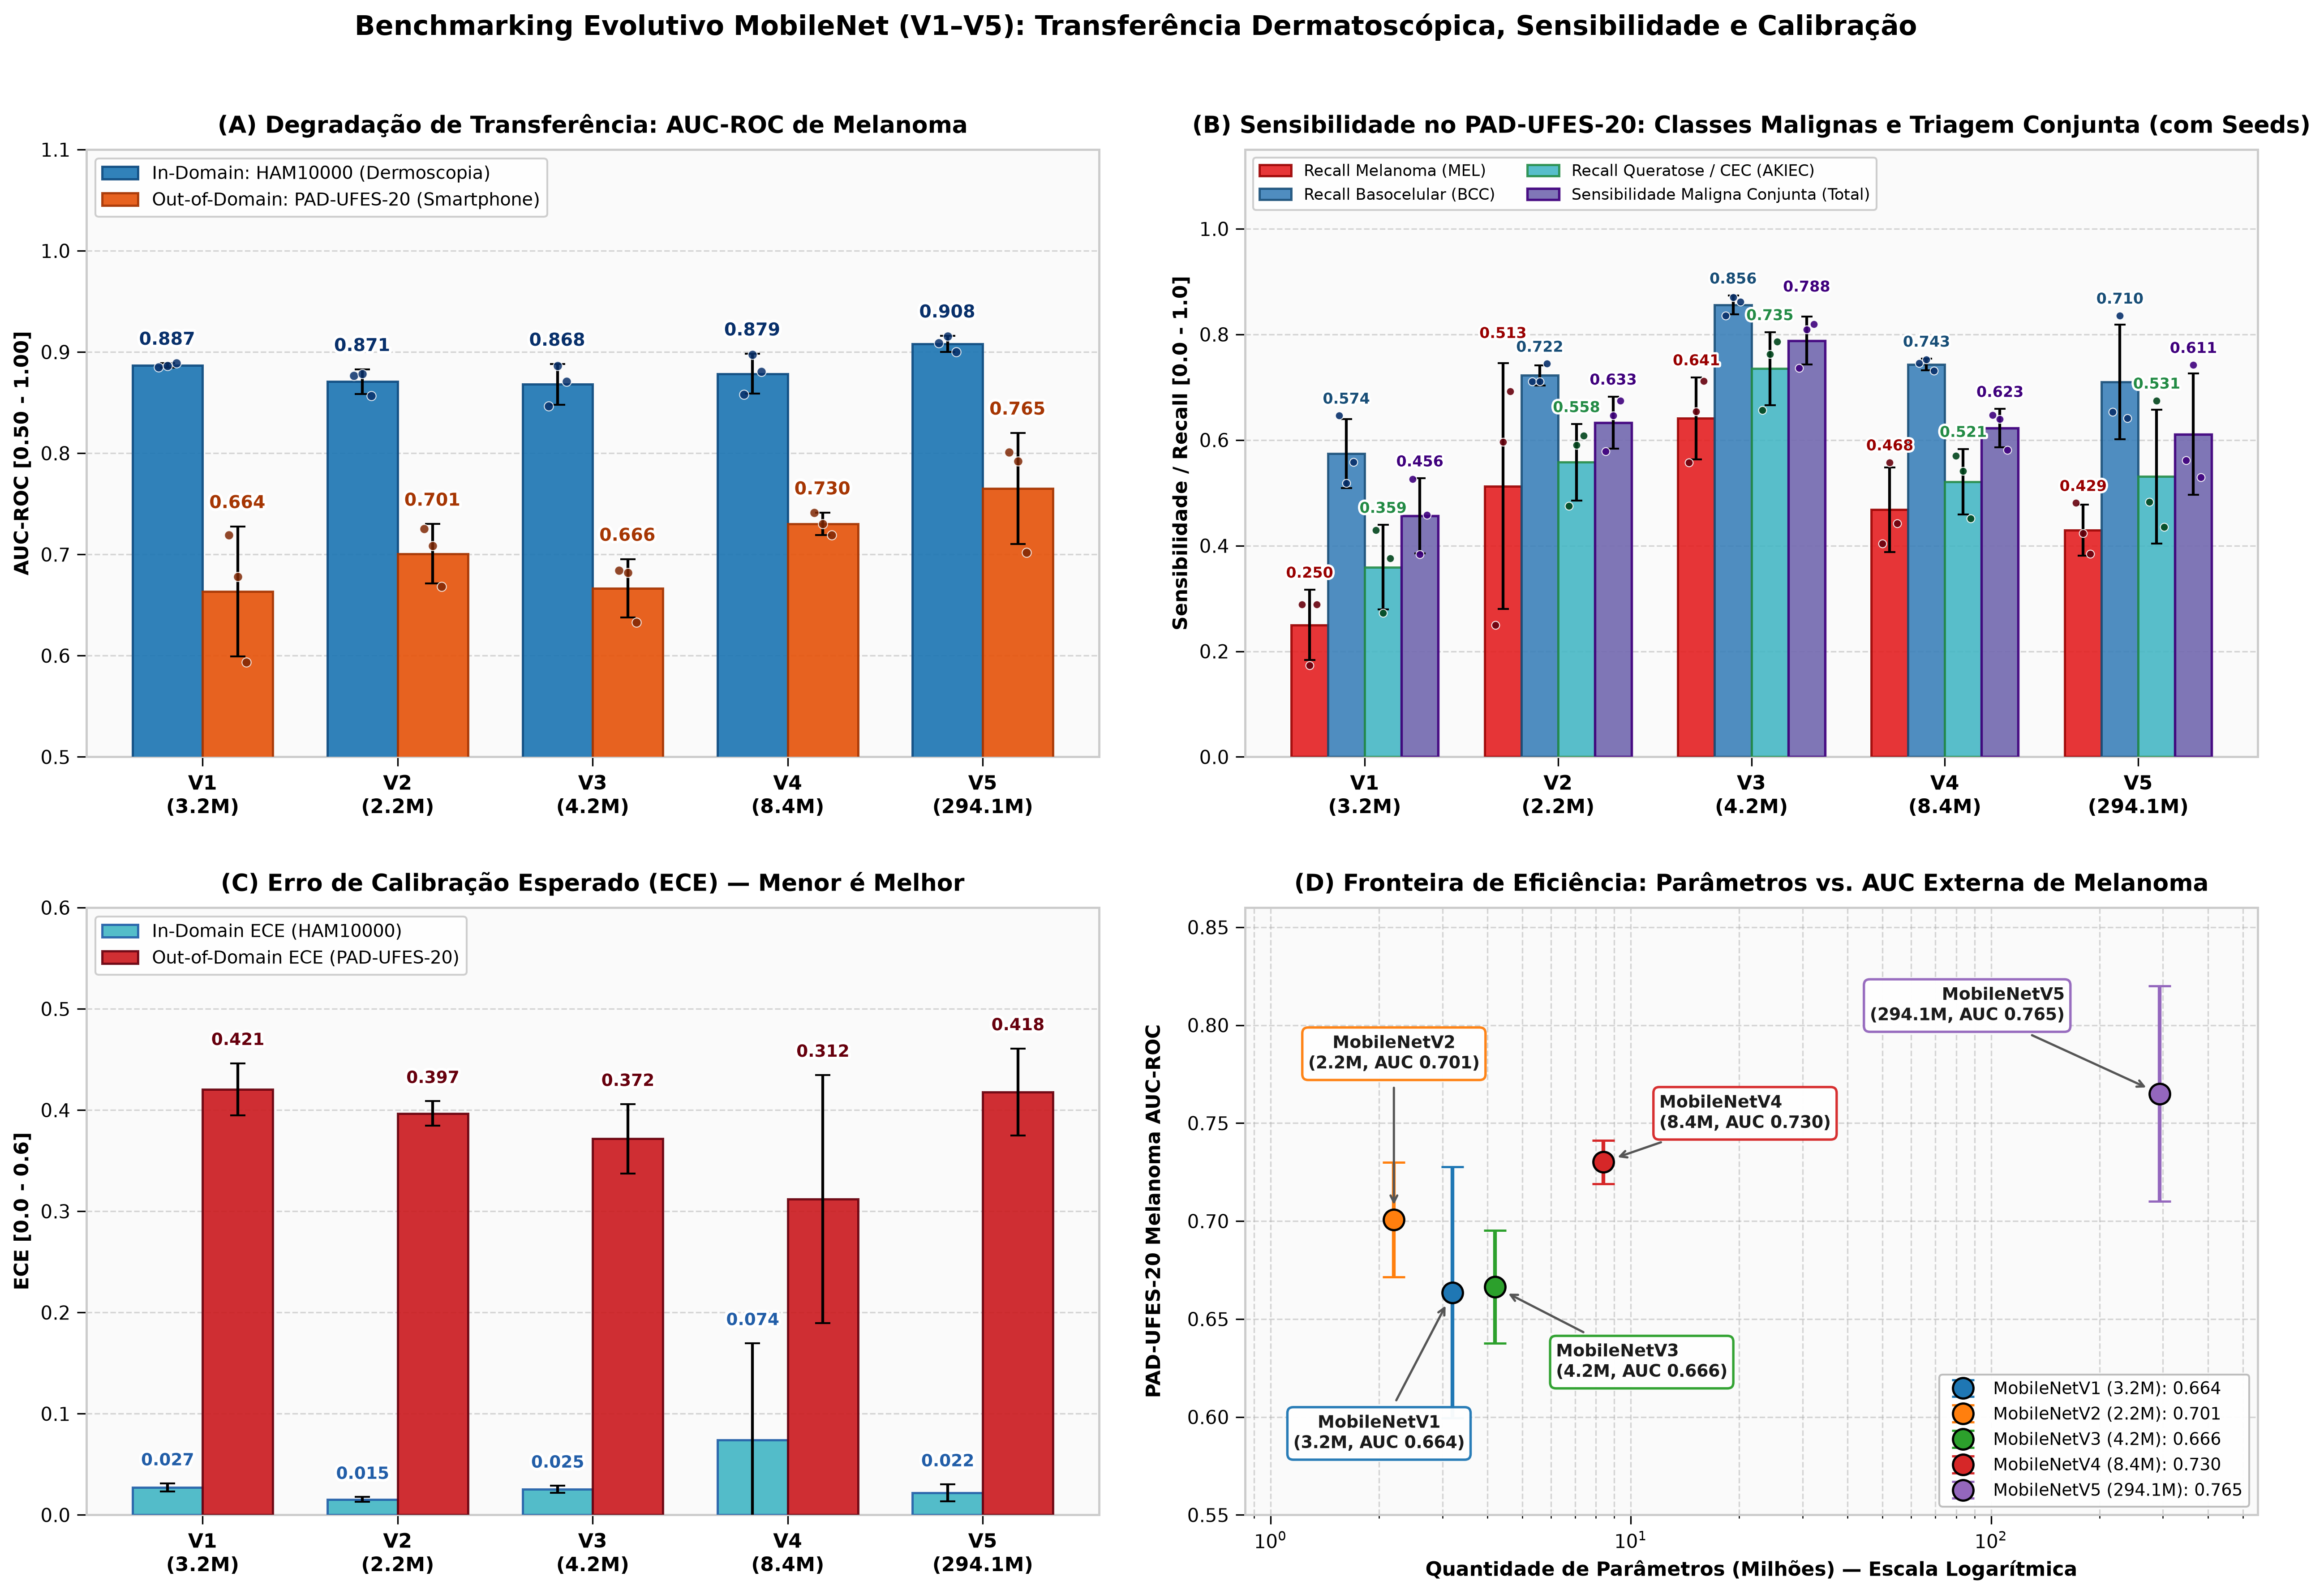
\includegraphics[width=\textwidth]{experiments/05_09_2026_run2/benchmark_comparison.png}
\caption{Comparação consolidada das arquiteturas nos domínios HAM10000 e PAD-UFES-20.}
\label{fig:benchmark}
\fonte{Elaborado pelo autor.}
\end{figure}

\section{Variação entre sementes}

A repetição mostrou que estabilidade interna não implica estabilidade externa. A V1 teve desvio-padrão de apenas 0,0017 na AUC de melanoma do HAM-test, mas 0,0523 no PAD-UFES-20. A V5 também foi estável no HAM-test, com desvio de 0,0064, e variável externamente, com desvio de 0,0449 na AUC de melanoma e 0,0936 na sensibilidade maligna.

Na V5, a semente 43 foi selecionada na época 10, enquanto as sementes 42 e 44 foram selecionadas nas épocas 20 e 39. A semente 43 alcançou PAD MEL AUC de 0,7018, abaixo de 0,7923 e 0,8010 nas outras execuções, mas obteve sensibilidade maligna de 0,7422, acima de 0,5618 e 0,5294. Isso demonstra que AUC e sensibilidade em um ponto operacional não são intercambiáveis e reforça a necessidade de reportar distribuições, em vez de escolher a melhor semente.

\section{Mudança de domínio}

Para V5, a AUC média de melanoma caiu de 0,9081 no HAM-test para 0,7650 no PAD-UFES-20. Como exemplo representativo, a semente 42 caiu de 0,9155 para 0,7923, diferença de 0,1232. O intervalo de confiança de 95\% da AUC externa nessa execução foi de 0,7315 a 0,8547. A amplitude é relevante porque o conjunto externo contém somente 52 melanomas.

O limiar de melanoma da mesma execução atingiu sensibilidade de 80,73\% no HAM-test e 48,08\% no PAD-UFES-20. A política \texttt{sens90} havia sido ajustada para alcançar 90\% no HAM-val; a redução em HAM-test já mostra erro de generalização interno, e a queda adicional no PAD evidencia alteração da distribuição. O limiar não foi reajustado no conjunto externo, preservando a independência da avaliação.

A classificação multiclasse também se degradou. Na execução V5/seed42, a acurácia restrita às cinco classes externas foi 26,41\%. Os \textit{recalls} de \textit{argmax} foram 7,16\% para AKIEC, 28,88\% para BCC e 28,85\% para melanoma, enquanto NV alcançou 93,9\%. A concentração de acertos em NV é compatível com dependência das características e priors do domínio fonte. Esses valores de \textit{recall} multiclasse não devem ser comparados diretamente com a sensibilidade de 48,08\% da triagem de melanoma, pois utilizam regras de decisão distintas. A distribuição dos erros diagnósticos e a predominância de predições direcionadas a nevos melanocíticos podem ser observadas nas matrizes de confusão da Figura~\ref{fig:confusoes-pad}.

\begin{figure}[H]
\centering
\begin{subfigure}[t]{0.49\textwidth}
\centering
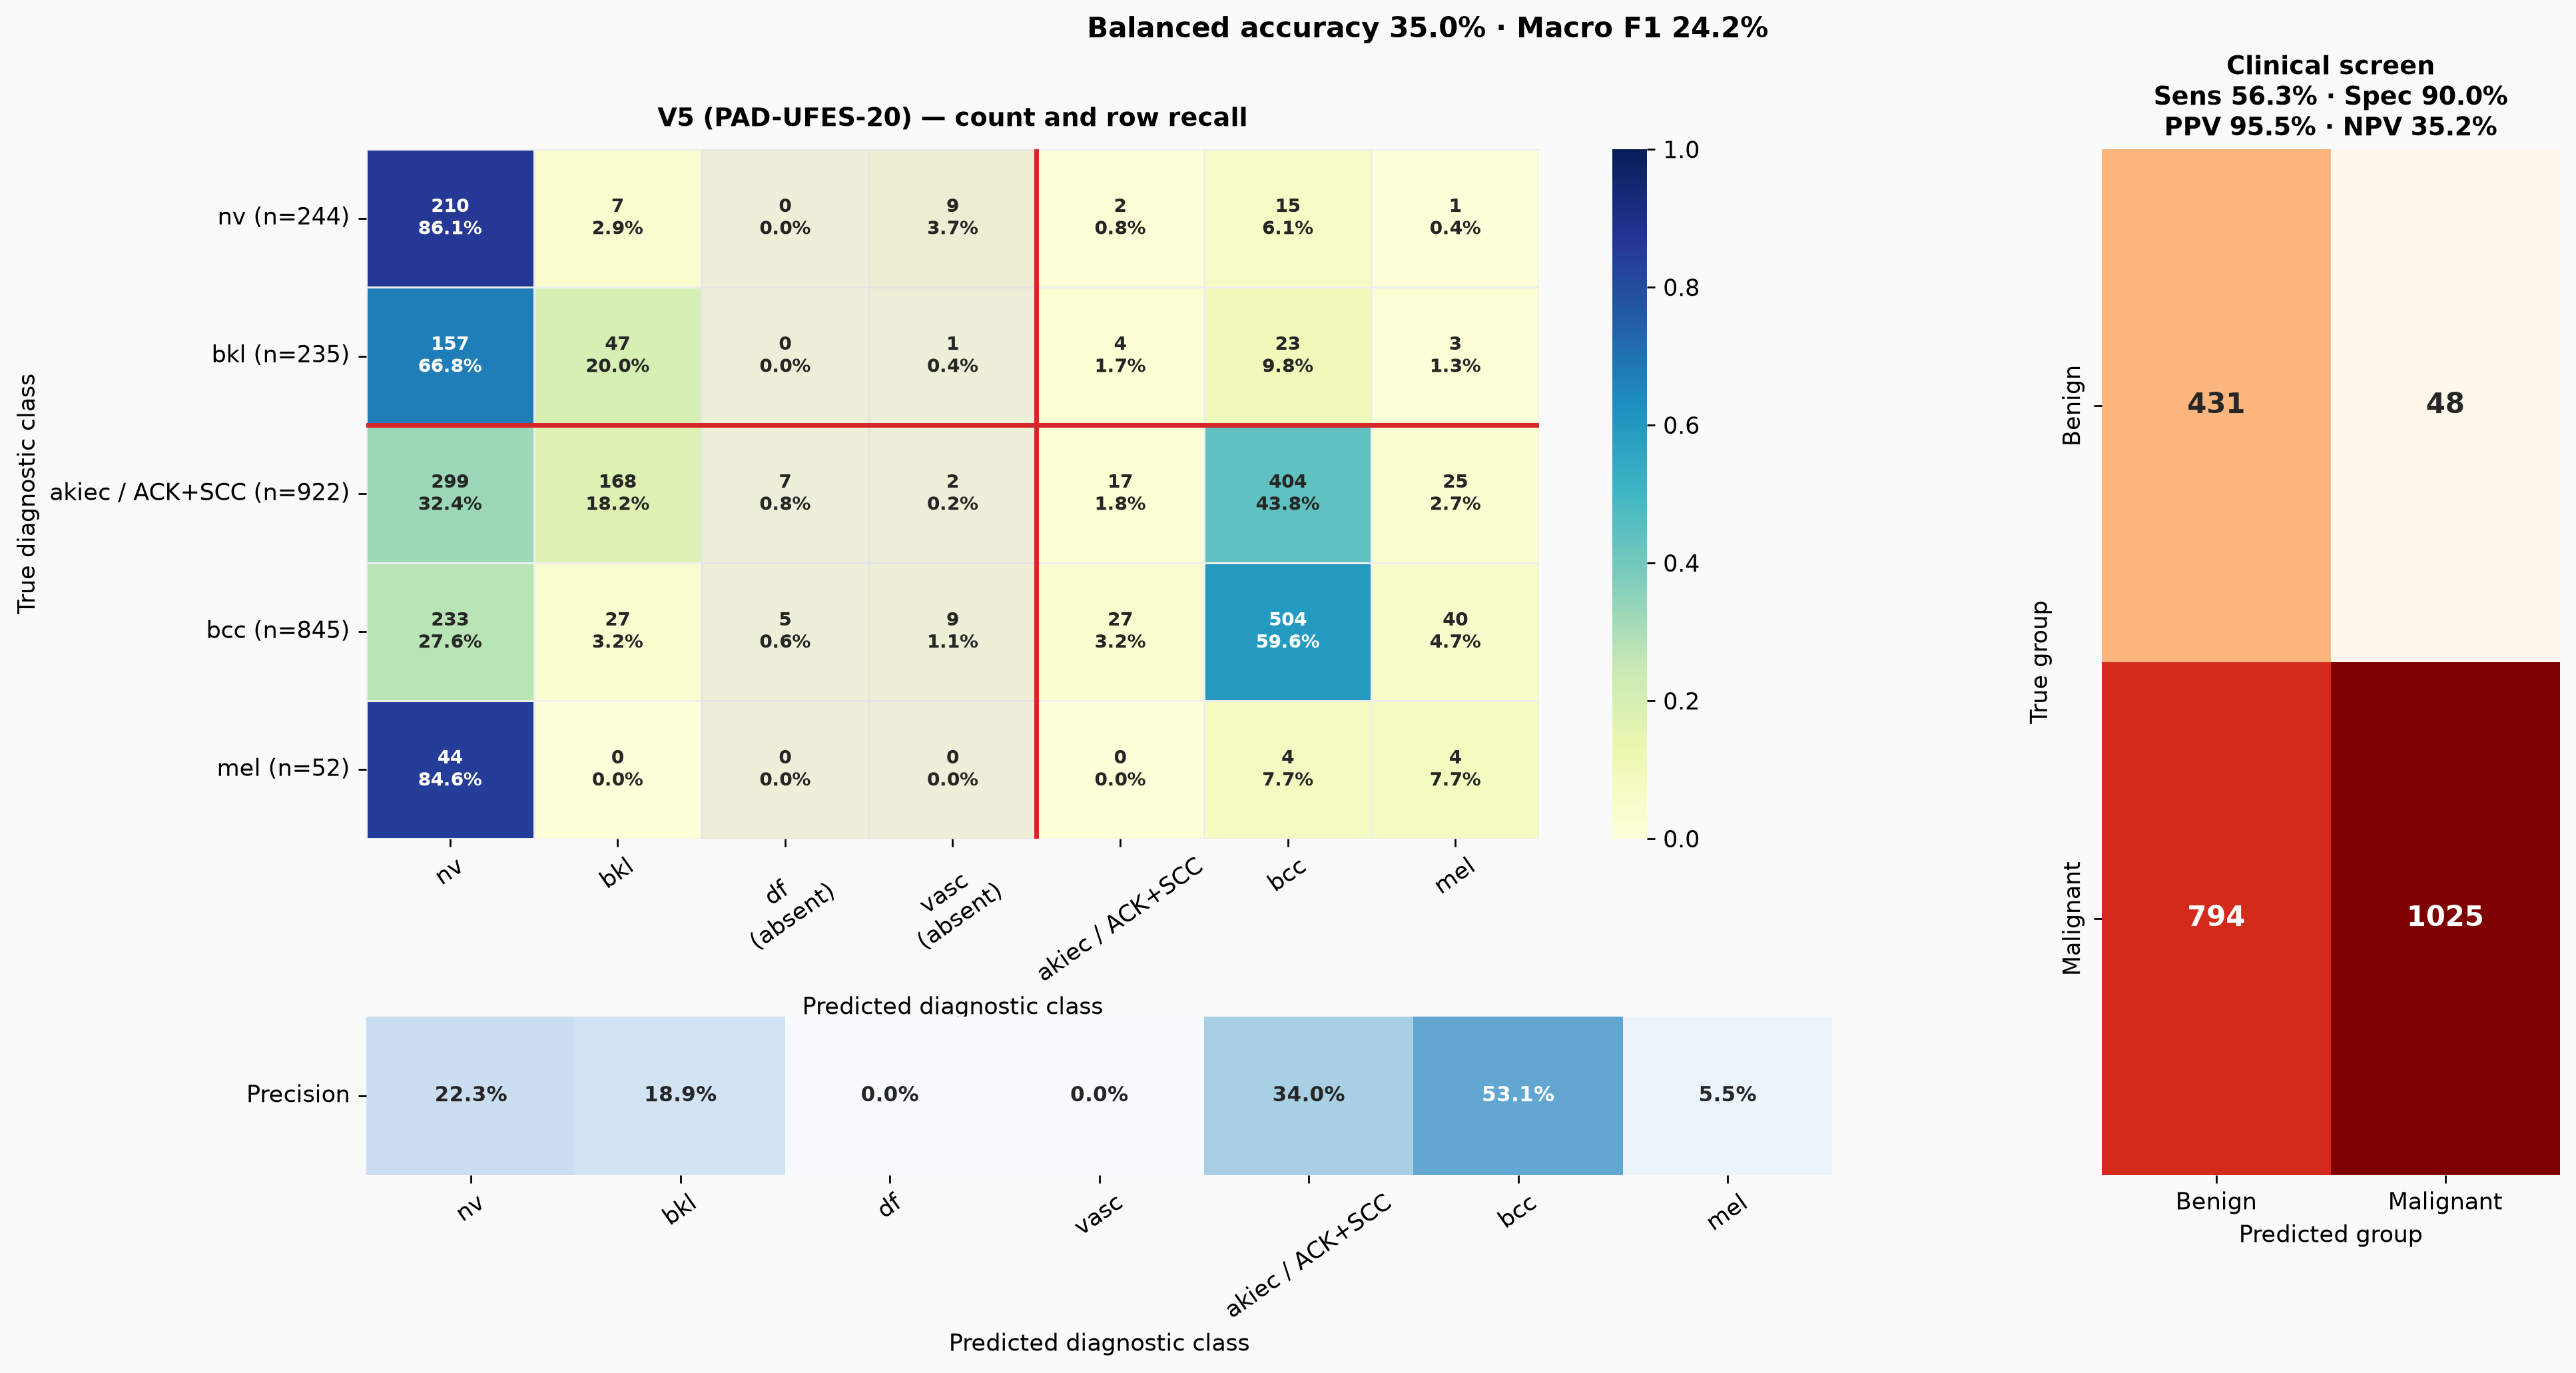
\includegraphics[width=\textwidth]{experiments/05_09_2026_run2/scenarios/main/v5/seed43/pad_ufes_20/confusion_matrix.png}
\caption{V5, semente 43.}
\end{subfigure}
\hfill
\begin{subfigure}[t]{0.49\textwidth}
\centering
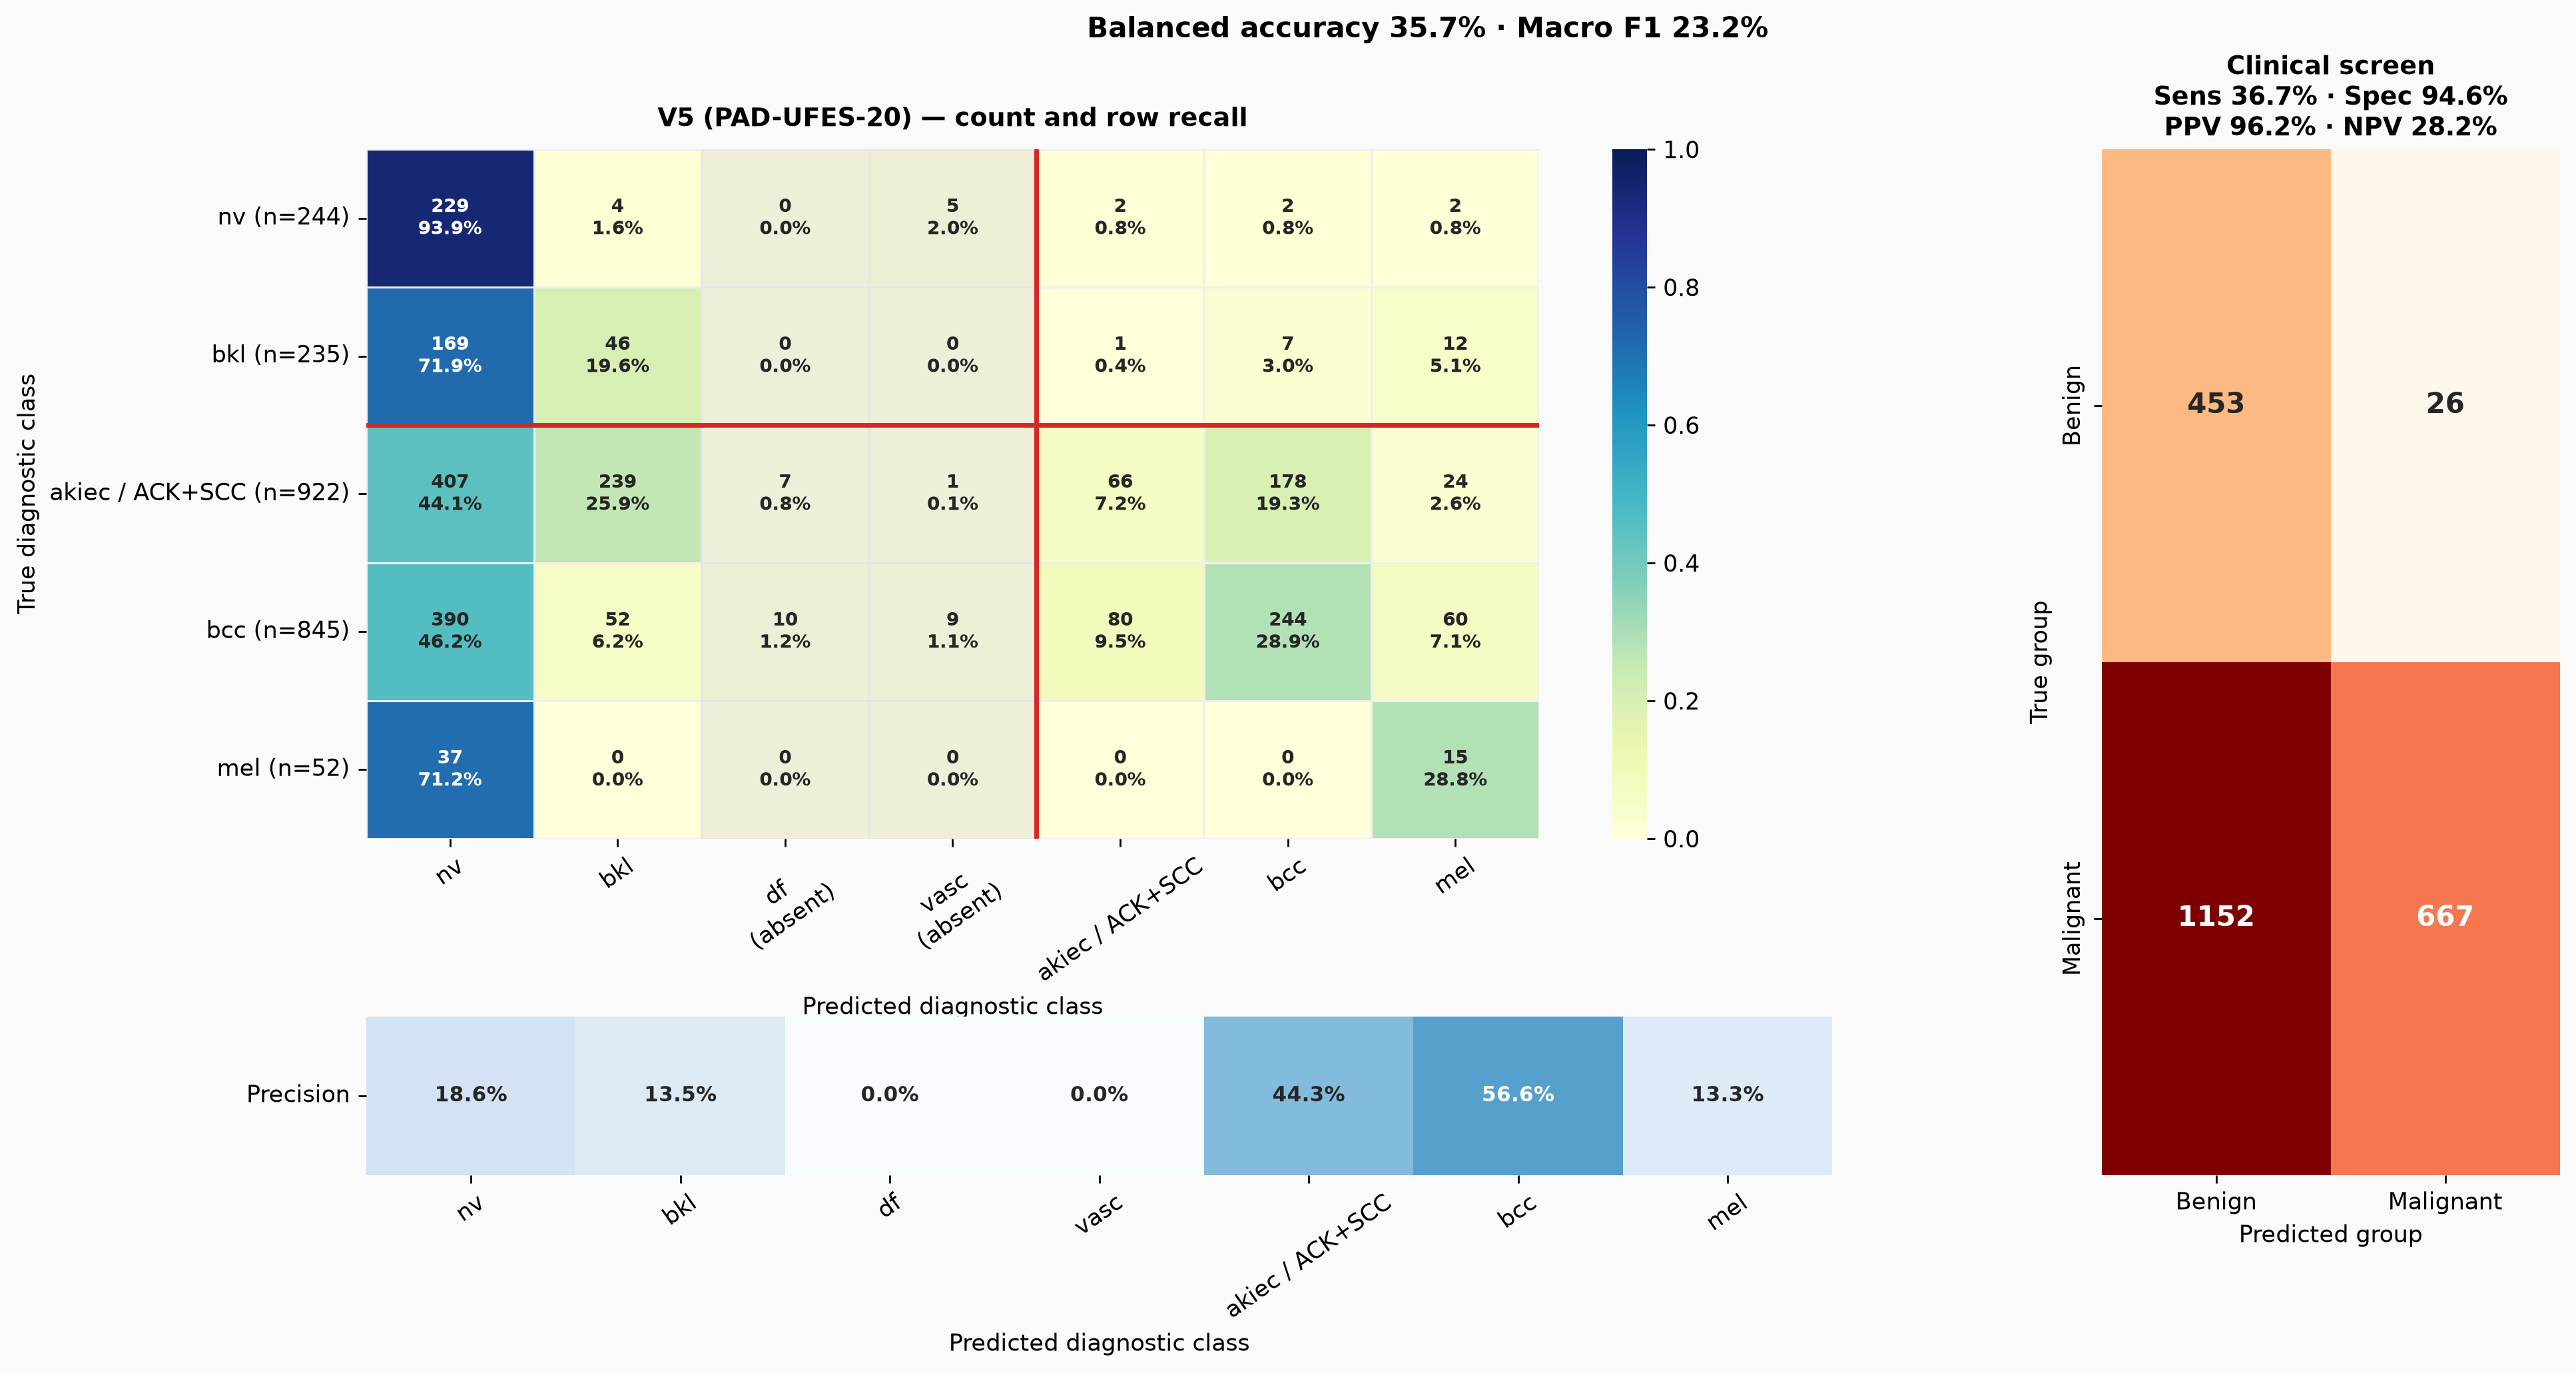
\includegraphics[width=\textwidth]{experiments/05_09_2026_run2/scenarios/main/v5/seed42/pad_ufes_20/confusion_matrix.png}
\caption{V5, semente 42.}
\end{subfigure}
\caption{Matrizes de confusão no PAD-UFES-20 para execuções representativas.}
\label{fig:confusoes-pad}
\fonte{Elaborado pelo autor.}
\end{figure}

\section{Calibração e regras de decisão}

Na V5/seed42, a temperatura $T=0{,}6565$ reduziu o ECE do HAM-val de 0,1156 para 0,0304. Após a mesma transformação, o ECE foi 0,0208 no HAM-test e 0,4399 no PAD-UFES-20. Nas três sementes da V5, o ECE externo pós-temperatura permaneceu em $0{,}4178\pm0{,}0352$. Portanto, o ajuste produziu baixo ECE nos dados HAM sob o estimador de 15 faixas, mas não produziu baixo ECE no PAD. Como não foi registrado o ECE do PAD antes da transformação, não se conclui se a temperatura melhorou ou piorou a calibração externa. O descolamento da calibração entre os domínios interno e externo está ilustrado nos diagramas de confiabilidade da Figura~\ref{fig:calibracao-v5}.

\begin{figure}[H]
\centering
\begin{subfigure}[t]{0.49\textwidth}
\centering
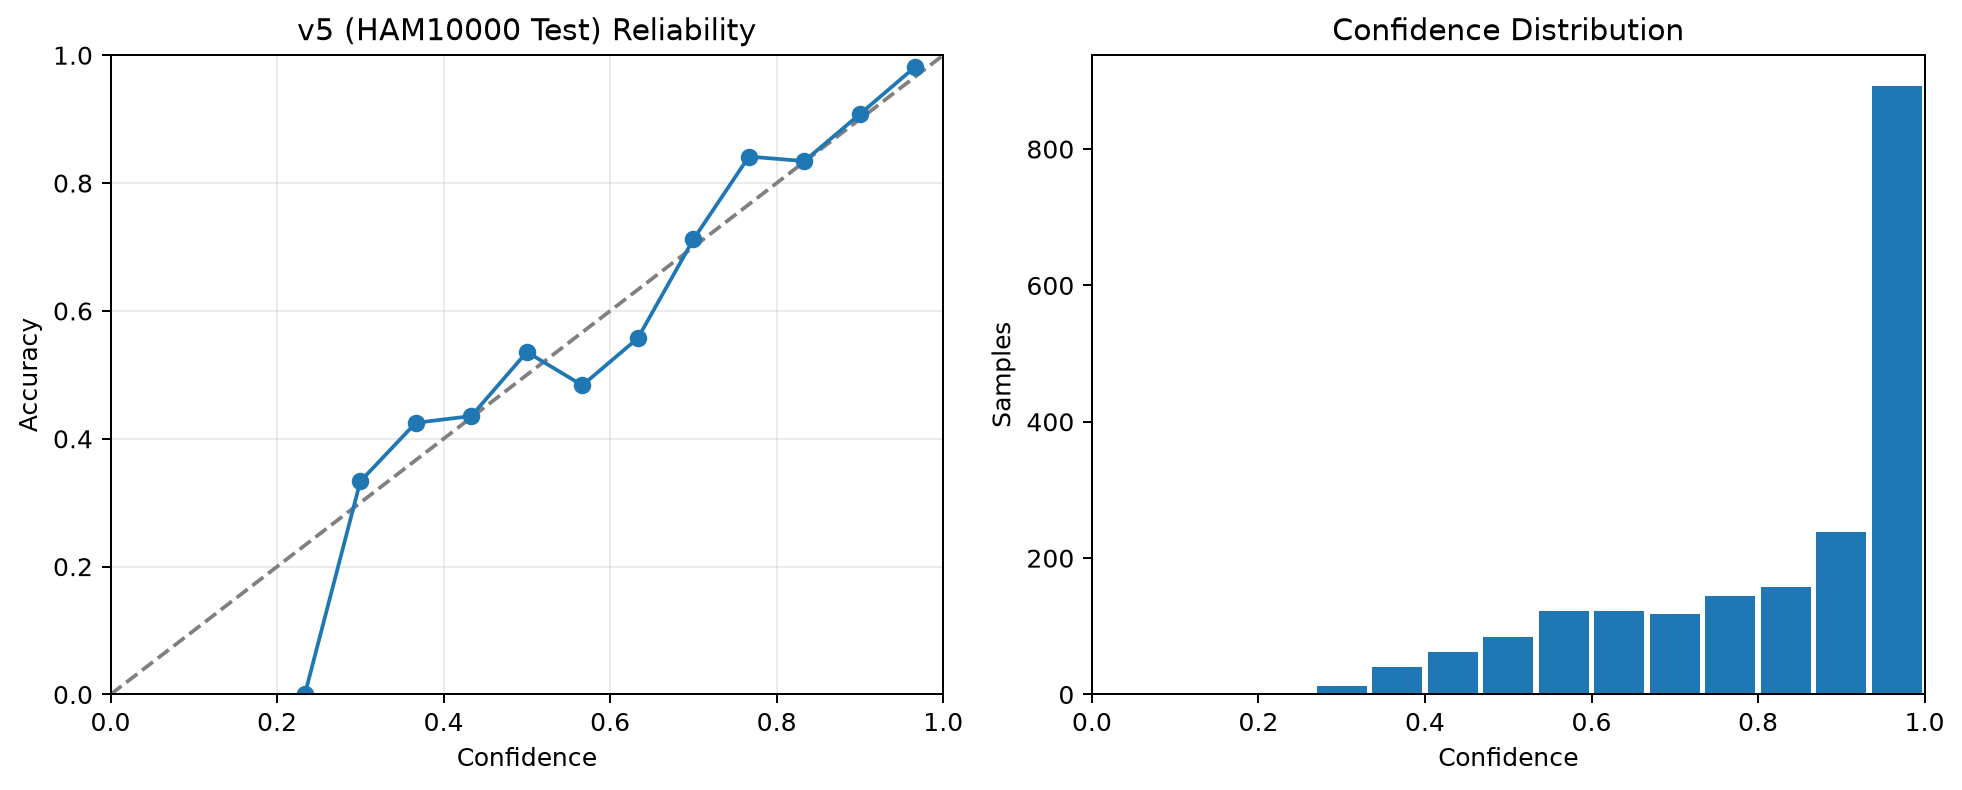
\includegraphics[width=\textwidth]{experiments/05_09_2026_run2/scenarios/main/v5/seed42/ham10000/reliability_diagram.png}
\caption{HAM-test.}
\end{subfigure}
\hfill
\begin{subfigure}[t]{0.49\textwidth}
\centering
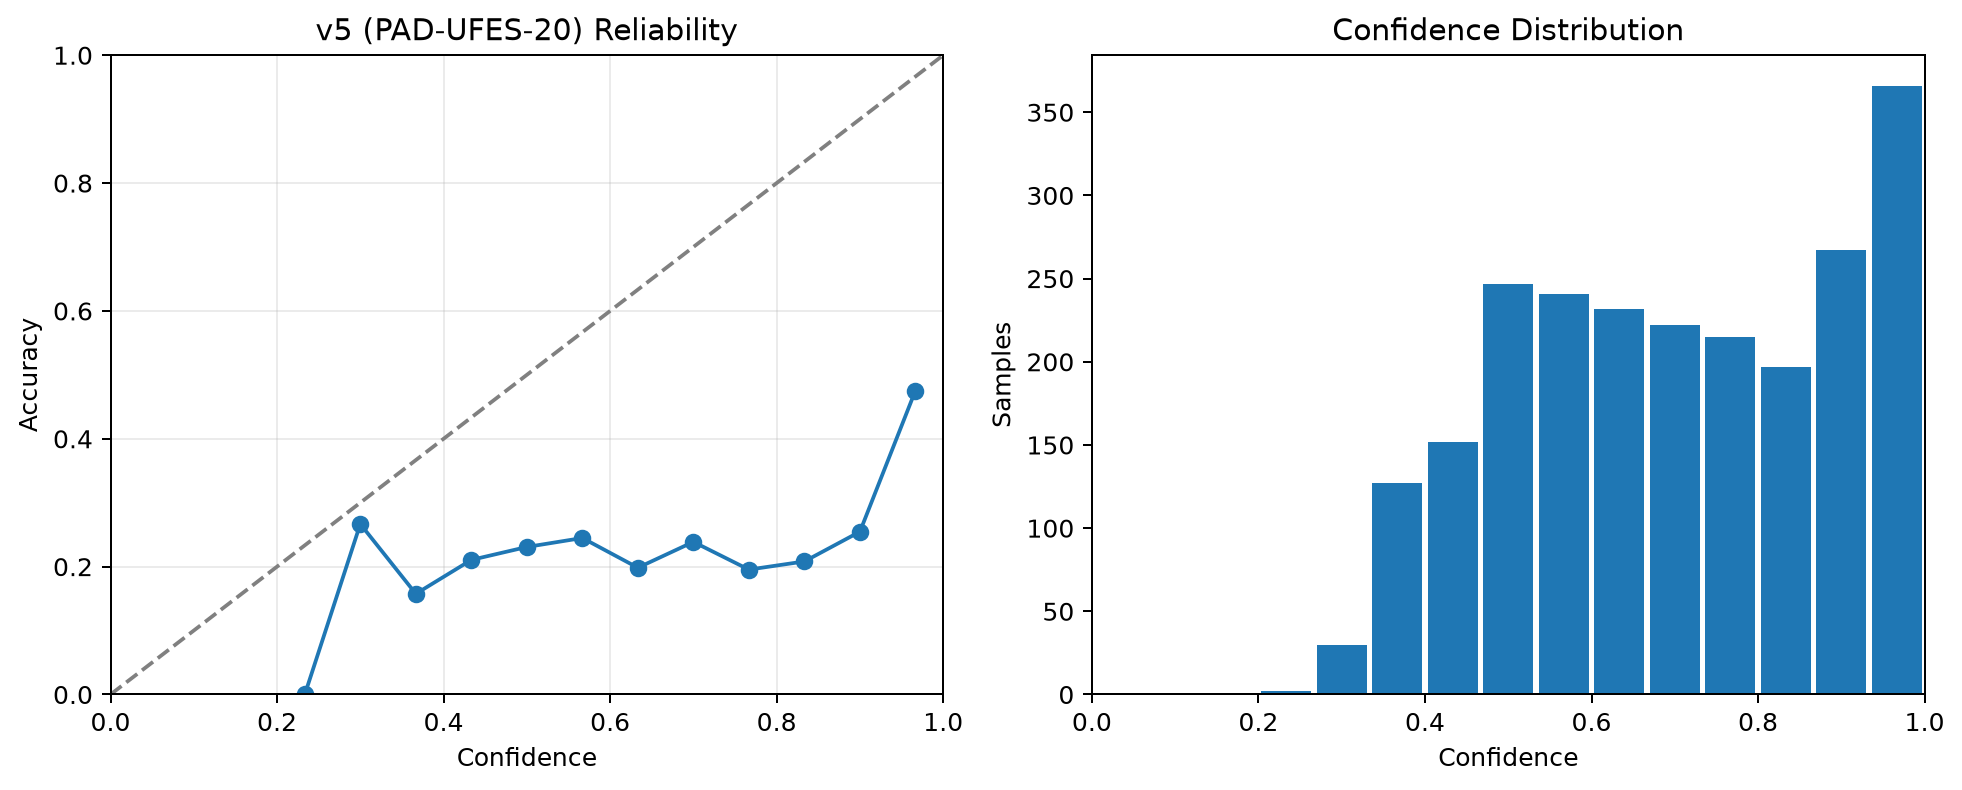
\includegraphics[width=\textwidth]{experiments/05_09_2026_run2/scenarios/main/v5/seed42/pad_ufes_20/reliability_diagram.png}
\caption{PAD-UFES-20.}
\end{subfigure}
\caption{Diagramas de confiabilidade da V5, semente 42. A temperatura foi estimada exclusivamente no HAM-val.}
\label{fig:calibracao-v5}
\fonte{Elaborado pelo autor.}
\end{figure}

Conforme modelado na Seção~\ref{sec:prior_correction_method} e no Apêndice~\ref{sec:apendice_prior_correction}, a correção de prior aumentou a acurácia balanceada no HAM-test em todas as médias das arquiteturas: V1, de 0,6511 para 0,7355; V2, de 0,6495 para 0,7139; V3, de 0,6486 para 0,7046; V4, de 0,6472 para 0,7169; e V5, de 0,6617 para 0,7342. No PAD-UFES-20, contudo, o efeito foi inconsistente entre as execuções. Como o hiperparâmetro de escala $\tau_{\text{prior}}$ foi selecionado estritamente no HAM-val, o resultado evidencia que o alinhamento empírico de probabilidades a priori calibrado no domínio fonte não é suficiente para neutralizar a severa quebra de prevalência epidemiológica (\textit{Prior Shift}) observada no cenário clínico real.

\section{Estudo de ablação}

As ablações foram comparadas somente com V3/seed42, mantendo arquitetura, divisão e semente. Cada configuração possui uma execução; portanto, as diferenças são indicativas e não permitem inferência estatística conclusiva. Os resultados desse ensaio de ablação estão consolidados na Tabela~\ref{tab:ablacao}.

\begin{table}[H]
\centering
\caption{Estudo de ablação da V3 com semente 42.}
\label{tab:ablacao}
\resizebox{\textwidth}{!}{
\begin{tabular}{lrrrr}
\toprule
Configuração & HAM MEL AUC & PAD MEL AUC & PAD macro AUC & PAD sens. maligna \\
\midrule
Completa & \textbf{0,8865} & 0,6821 & \textbf{0,6946} & \textbf{0,7367} \\
Sem perda focal & 0,8711 & \textbf{0,7145} & 0,6914 & 0,6531 \\
Sem Mixup & 0,8494 & 0,6971 & 0,6845 & 0,6449 \\
Sem amostrador balanceado & 0,8156 & 0,6317 & 0,6521 & 0,5717 \\
\bottomrule
\end{tabular}}
\fonte{Elaborado pelo autor.}
\end{table}

A retirada do amostrador produziu, na única semente avaliada, a maior deterioração conjunta observada: queda de 0,0709 na AUC de melanoma do HAM-test, 0,0504 na AUC de melanoma externa, 0,0425 na AUC macro externa e 0,1650 na sensibilidade maligna. Esse contraste não estima um efeito causal ou reproduzível sem repetição em outras sementes.

A remoção da perda focal reduziu discriminação interna e sensibilidade maligna, mas aumentou a AUC externa de melanoma de 0,6821 para 0,7145. A remoção do Mixup também produziu AUC externa de melanoma superior à configuração completa, porém piorou AUC interna, AUC macro externa e sensibilidade maligna. Como cada ablação tem $n=1$, não se conclui que perda focal ou Mixup reduzam sistematicamente a transferência de melanoma; o resultado pode incluir variação estocástica.

\section{Custo estrutural e escopo de implantação}

A ordenação por parâmetros foi V2 (2,2 M), V1 (3,2 M), V3 (4,2 M), V4 (8,4 M) e V5 (294,1 M). V5 obteve a maior discriminação média observada. Seu número de parâmetros sugere maior custo de armazenamento que V1--V4, mas não permite concluir sobre adequação à borda. A V4 foi aproximadamente 35 vezes menor e apresentou a maior AUC externa média observada de melanoma entre as arquiteturas compactas. A V3 foi menor que a V4 e apresentou a maior sensibilidade maligna média observada.

O número de parâmetros não determina sozinho tamanho quantizado, latência, memória de pico, consumo energético ou compatibilidade de operadores. Como essas dimensões não foram medidas, não se afirma que qualquer modelo esteja pronto para smartphone. Exportação, quantização e \textit{benchmark} no dispositivo permanecem trabalhos futuros.

\section{Análise qualitativa de interpretabilidade}

Os mapas de explicabilidade visual (Grad-CAM para V4 e LayerCAM para V5) permitem comparar as regiões de atenção espacial do modelo em fotografias clínicas reais. A análise qualitativa avalia casos representativos de verdadeiros positivos, falsos negativos e falsos positivos, verificando se a ativação da rede se concentra na morfologia patológica da lesão ou em elementos espúrios de fundo (como bordas de fita, réguas e pelos), conforme ilustrado na Figura~\ref{fig:gradcam-pad}. Os mapas não constituem explicação causal nem validação clínica formal.

\begin{figure}[H]
\centering
\begin{subfigure}[t]{0.49\textwidth}
\centering
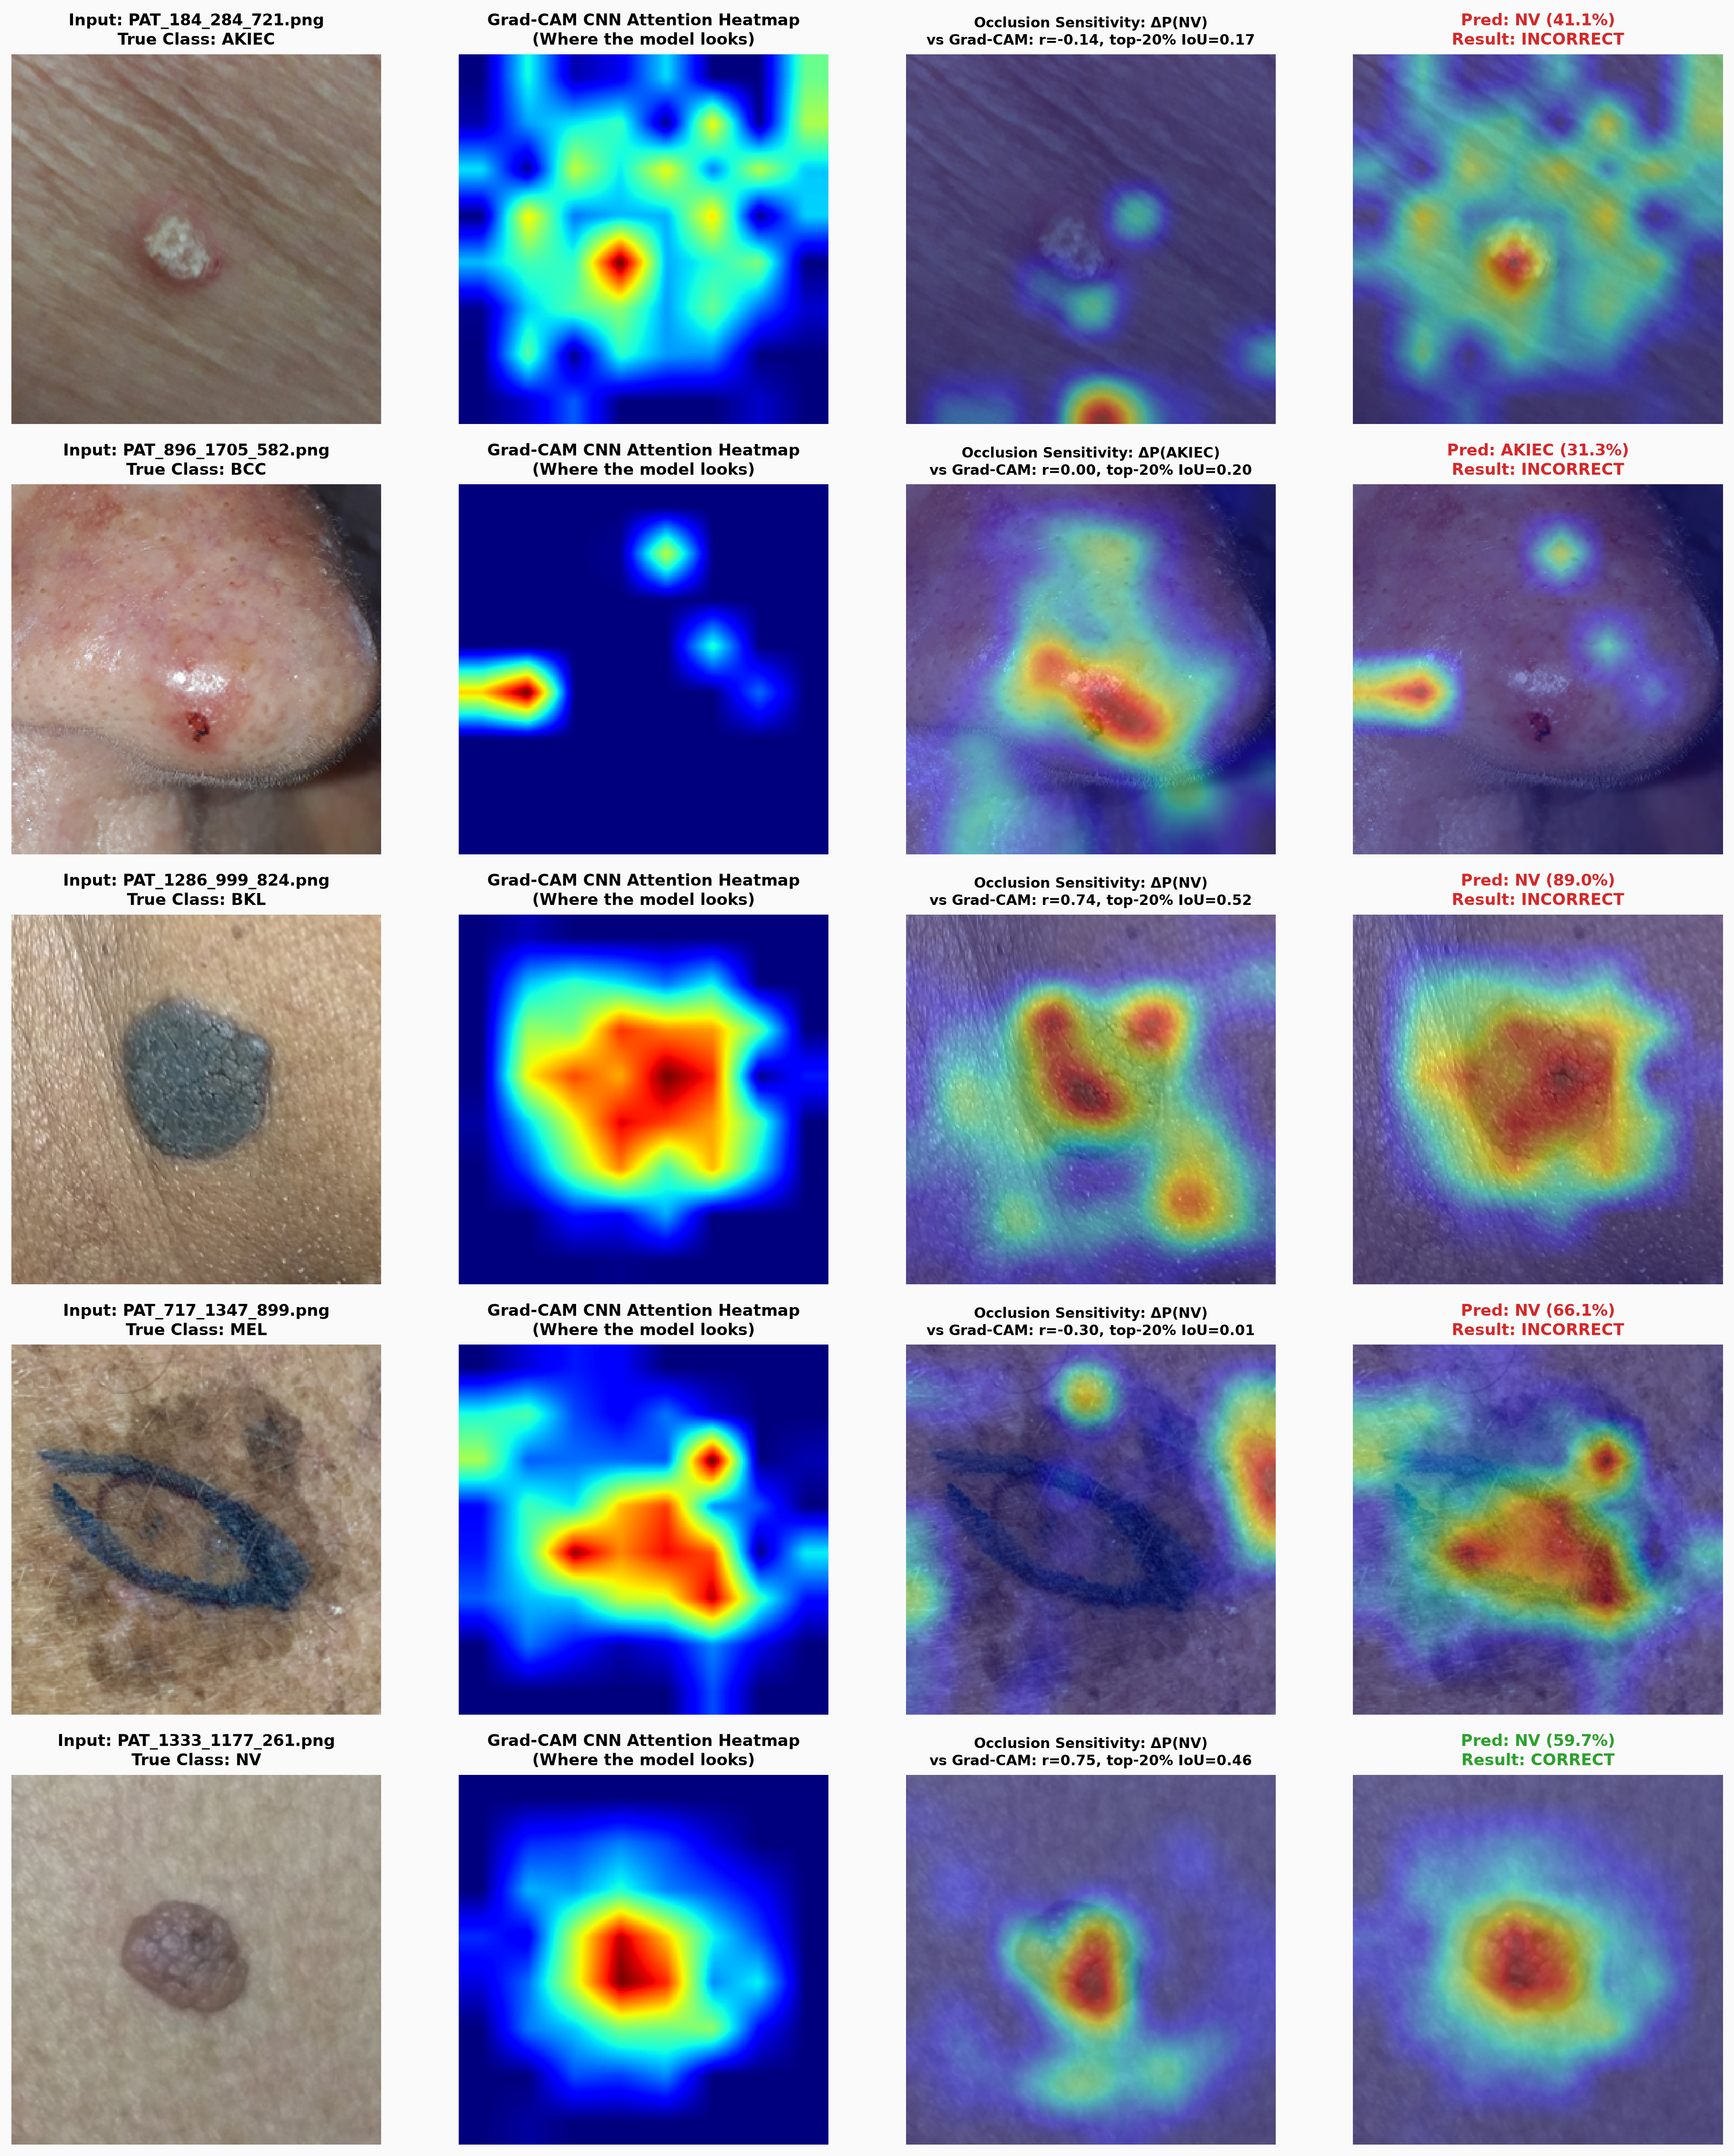
\includegraphics[width=\textwidth]{experiments/05_09_2026_run2/scenarios/main/v4/seed43/pad_ufes_20/gradcam_heatmaps.png}
\caption{V4, semente 43 (Grad-CAM).}
\end{subfigure}
\hfill
\begin{subfigure}[t]{0.49\textwidth}
\centering
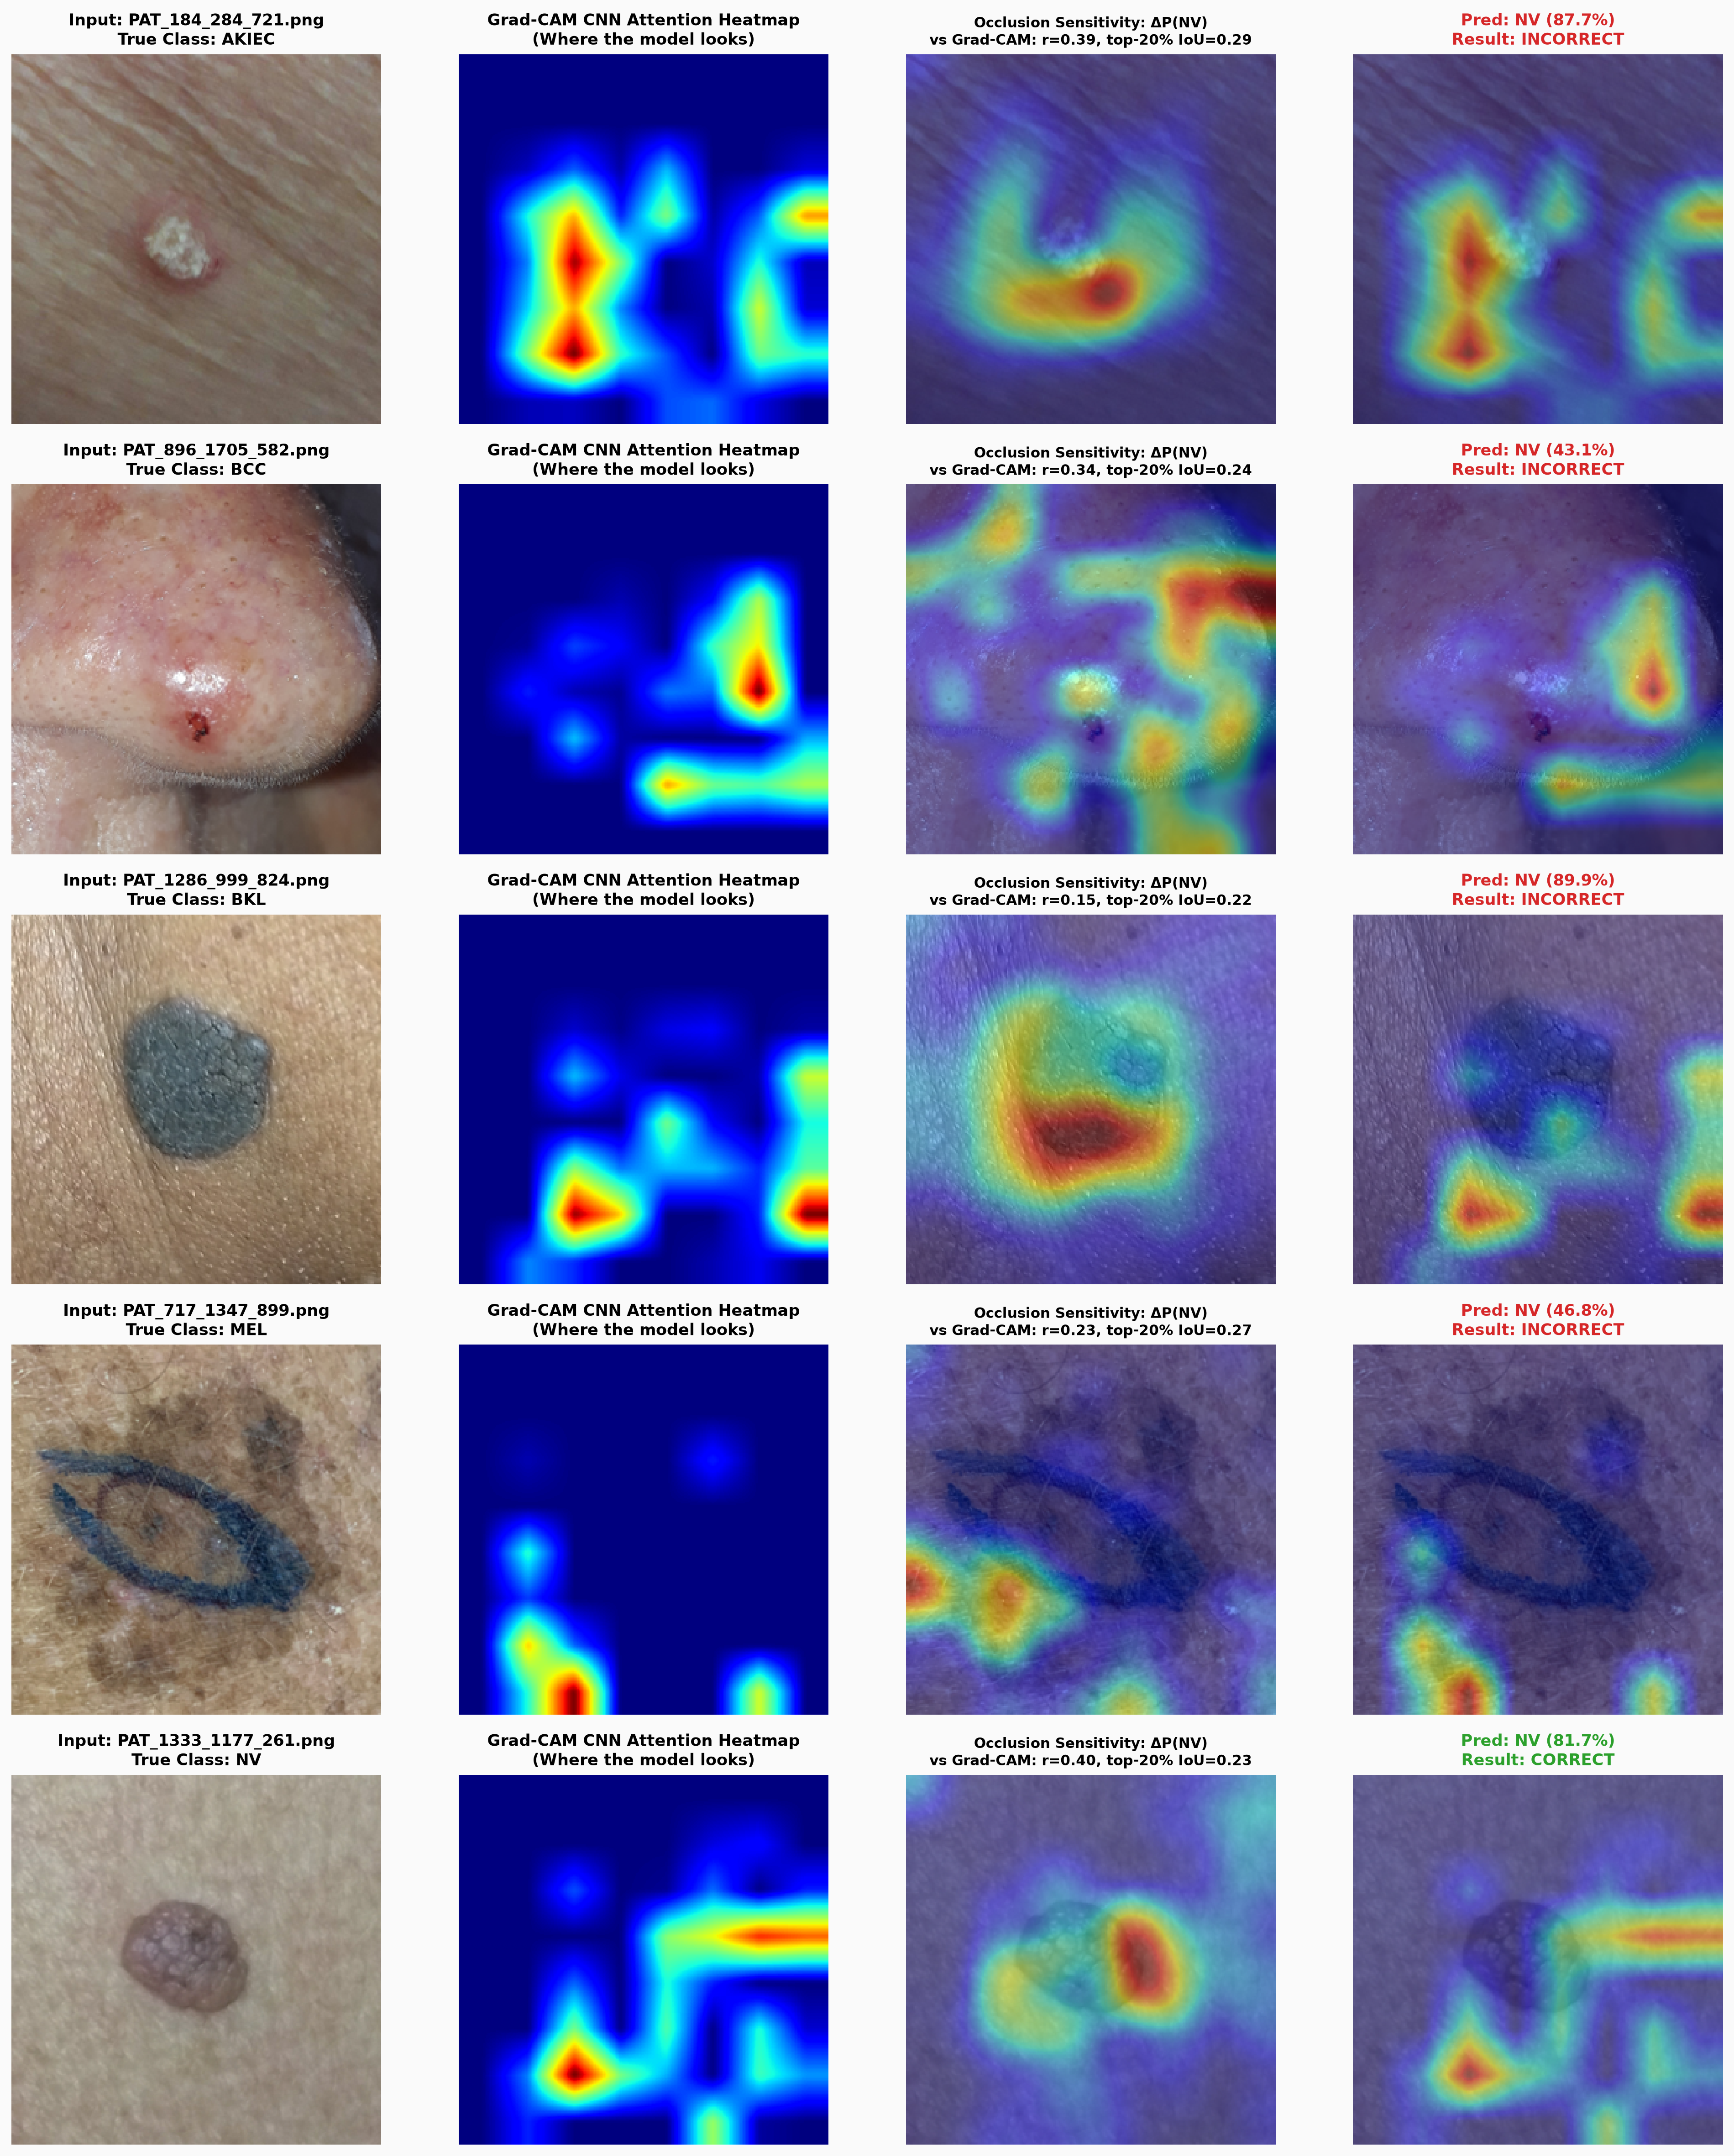
\includegraphics[width=\textwidth]{experiments/05_09_2026_run2/scenarios/main/v5/seed42/pad_ufes_20/gradcam_heatmaps.png}
\caption{V5, semente 42 (LayerCAM).}
\end{subfigure}
\caption{Galerias de explicabilidade visual no PAD-UFES-20 (Grad-CAM para V4 e LayerCAM para V5). A interpretação deve permanecer qualitativa.}
\label{fig:gradcam-pad}
\fonte{Elaborado pelo autor.}
\end{figure}

\section{Limitações}

\begin{itemize}
    \item Três sementes por arquitetura caracterizam dispersão inicial, mas não sustentam comparações estatísticas fortes.
    \item As ablações possuem somente uma semente e seus efeitos não são conclusivos.
    \item O PAD-UFES-20 contém somente 52 melanomas, de modo que poucos casos alteram substancialmente a sensibilidade.
    \item A união de ACK e SCC em AKIEC é taxonomicamente pragmática, porém clinicamente imperfeita.
    \item A comparação HAM--PAD altera simultaneamente modalidade, população, prevalência e condições de captura; o experimento não isola a causa de cada queda.
    \item O PAD-UFES-20 é independente do treinamento e da calibração, mas foi utilizado para comparar arquiteturas. Um terceiro conjunto clínico intocado seria necessário para confirmar uma escolha feita a partir destes resultados.
    \item Não houve treinamento PAD-only, treinamento misto nem adaptação HAM--PAD; os resultados não demonstram que treinamento exclusivo no HAM10000 seja a melhor estratégia de implantação.
    \item Não foram medidos latência, memória, consumo energético ou desempenho quantizado em dispositivo.
\end{itemize}

\section{Síntese dos resultados}

Em resposta à questão de pesquisa, as representações aprendidas no HAM10000 preservaram parte da capacidade de discriminar melanoma no PAD-UFES-20, mas não preservaram de modo confiável baixo ECE, classificação multiclasse ou sensibilidade nos limiares transferidos. Na comparação exploratória, a V5 exibiu a maior discriminação média observada, com 294,1 milhões de parâmetros. Segundo número de parâmetros e médias observadas, a V4 constituiu um compromisso descritivo entre os modelos menores para discriminação de melanoma. A V3 apresentou a maior sensibilidade média observada da triagem conjunta de malignidade. Essas preferências precisam ser confirmadas em um terceiro conjunto clínico.

A mudança de domínio foi observada em todas as arquiteturas e foi especialmente clara na calibração externa. Assim, AUC elevada no domínio fonte não é evidência suficiente de segurança no domínio clínico. Nenhum dos modelos avaliados pode ser considerado pronto para implantação ou uso diagnóstico a partir destes resultados isolados.

\chapter{Conclusão}

O trabalho implementou e avaliou um pipeline auditável de treinamento multiclasse e triagem derivada para lesões cutâneas. A separação por identificador de lesão, o teste interno reservado, a avaliação externa sem adaptação, a repetição em sementes e os intervalos de confiança fortaleceram o desenho em comparação com uma avaliação baseada em uma única divisão ou em acurácia simples.

Os resultados mostraram três compromissos descritivos na comparação exploratória. V5 ofereceu a maior discriminação média observada, porém é muito maior e apresentou ECE externo elevado. V4 ofereceu a maior AUC externa média observada de melanoma entre os modelos compactos, enquanto a V3 ofereceu a maior sensibilidade média observada de triagem maligna. Na única semente da ablação, a retirada da amostragem balanceada coincidiu com a deterioração conjunta mais clara, sem estabelecer um efeito causal reproduzível.

A principal conclusão é que desempenho dermatoscópico não pode ser transferido diretamente para imagens clínicas sem validação específica. Limiar ajustado para sensibilidade no HAM-val não garantiu a mesma sensibilidade no PAD-UFES-20, e a temperatura ajustada internamente não preservou calibração. Esses resultados limitam qualquer alegação de aplicação clínica imediata.

Como continuidade e desdobramento desta pesquisa, apontam-se as seguintes frentes de trabalhos futuros:
\begin{itemize}
    \item \textbf{Validação Clínica e Adaptação de Domínio:} Avaliar as redes em uma terceira base clínica multicêntrica e investigar técnicas de Adaptação de Domínio Não Supervisionada (\textit{Unsupervised Domain Adaptation}), reduzindo o impacto da quebra de distribuição entre dermatoscopia e fotos de celulares;
    \item \textbf{Quantização e Perfilamento Físico de Borda:} Realizar a conversão dos modelos selecionados (como a MobileNetV3 e V4) para formatos portáveis (ONNX / TFLite) através de Quantização Pós-Treinamento em precisão inteira (INT8 PTQ), mensurando em dispositivos físicos reais a latência de inferência (em milissegundos), o consumo de pico de memória RAM e a eficiência energética;
    \item \textbf{Desenvolvimento do Aplicativo Móvel:} Implementar uma prova de conceito de aplicativo móvel (para os sistemas operacionais Android ou iOS) que incorpore o modelo quantizado localmente, viabilizando a captura de imagens pela câmera e a execução de inferência diagnóstica 100\% \textit{offline}, sem qualquer dependência de conectividade com a internet ou servidores em nuvem;
    \item \textbf{Auditoria Estatística e Estudo de Ablação Expandido:} Conduzir experimentos de ablação em múltiplas sementes para isolar de forma causal e conclusiva os efeitos de componentes individuais de perda e regularização.
\end{itemize}

%=======================================================================
% Referências
%=======================================================================
\nocite{gemini2026}
\bibliography{exemplo}

%=======================================================================
% Exemplo de Apêndice
% O Apêndice é utilizado para apresentar material complementar elaborado
% pelo próprio autor.  Deve seguir as mesmas regras de formatação do
% corpo principal do documento.
%=======================================================================
\appendix
\chapter{Formulação Matemática e Operadores Analíticos}
\label{apendice:formulacao_matematica}

Este apêndice compila as formulações matemáticas, funções de custo e regras de decisão analíticas que fundamentam o pipeline experimental. As deduções estão organizadas cronologicamente conforme a execução do modelo.

\section{Harmonização Taxonômica e Espaço Amostral}
\label{sec:apendice_harmonizacao}

Os domínios HAM10000 e PAD-UFES-20 possuem os respectivos espaços de rótulos:
$$ \mathcal{Y}_{\text{HAM}} = \{\text{akiec}, \text{bcc}, \text{bkl}, \text{df}, \text{mel}, \text{nv}, \text{vasc}\} $$
$$ \mathcal{Y}_{\text{PAD}} = \{\text{ACK}, \text{BCC}, \text{MEL}, \text{NEV}, \text{SCC}, \text{SEK}\} $$

A função de mapeamento patológico por partes $M: \mathcal{Y}_{\text{PAD}} \to \mathcal{Y}_{\text{HAM}}$ compatibiliza os domínios para o subespaço compartilhado $C_{\text{shared}}$:
\begin{equation}
    \label{eq:apendice_mapeamento_taxonomico}
    M(y) = 
    \begin{cases}
        \text{akiec}, & \text{se } y \in \{\text{ACK}, \text{SCC}\}, \\
        \text{bkl},   & \text{se } y = \text{SEK}, \\
        \text{nv},    & \text{se } y = \text{NEV}, \\
        \text{mel},   & \text{se } y = \text{MEL}, \\
        \text{bcc},   & \text{se } y = \text{BCC}.
    \end{cases}
\end{equation}

A normalização bayesiana para a probabilidade condicional a posteriori sobre $C_{\text{shared}}$ anula a massa de probabilidade das classes ausentes (DF e VASC):
\begin{equation}
    \label{eq:apendice_prob_condicional}
    P(y = c \mid \mathbf{x}, y \in C_{\text{shared}}) = \frac{p_c}{\sum_{k \in C_{\text{shared}}} p_k}
\end{equation}

O desacoplamento prognóstico (\textit{Dual-Perspective}) define duas frentes operacionais:
\begin{align}
    \text{Focal (Melanoma):} \quad & P(\text{MEL} \mid \mathbf{x}) = p_{\text{mel}} \label{eq:apendice_projecao_melanoma} \\
    \text{Conjunta (Maligna):} \quad & P(\text{Maligna} \mid \mathbf{x}) = p_{\text{mel}} + p_{\text{bcc}} + p_{\text{akiec}} \label{eq:apendice_projecao_maligna}
\end{align}

\section{Interpolação Estocástica (Batch Mixup)}
\label{sec:apendice_mixup}

Para pares de instâncias $(\mathbf{x}_i, \mathbf{y}_i)$ e $(\mathbf{x}_j, \mathbf{y}_j)$, o algoritmo \textit{Mixup} \cite{zhang2018mixup} interpola as amostras através de um coeficiente escalar $\lambda$ amostrado de uma distribuição Beta simétrica:
\begin{equation}
    \label{eq:apendice_mixup_beta}
    \lambda \sim \operatorname{Beta}(\alpha, \alpha), \quad \alpha = 0{,}2
\end{equation}

A combinação linear convexa das entradas e dos rótulos \textit{one-hot} é dada por:
\begin{align}
    \tilde{\mathbf{x}} &= \lambda \mathbf{x}_i + (1 - \lambda) \mathbf{x}_j \label{eq:apendice_mixup_input} \\
    \tilde{\mathbf{y}} &= \lambda \mathbf{y}_i + (1 - \lambda) \mathbf{y}_j \label{eq:apendice_mixup_label}
\end{align}

A função de perda do modelo $f_\theta$ sobre os dados sintéticos é:
\begin{equation}
    \label{eq:apendice_mixup_loss}
    \mathcal{L}_{\text{mixup}} = \lambda \, \mathcal{L}\left(f_\theta(\tilde{\mathbf{x}}), \mathbf{y}_i\right) + (1 - \lambda) \, \mathcal{L}\left(f_\theta(\tilde{\mathbf{x}}), \mathbf{y}_j\right)
\end{equation}

\section{Aumento de Dados em Tempo de Teste (TTA)}
\label{sec:apendice_tta}

Conforme fundamentado nos estudos de aumento de dados \cite{shorten2019survey}, seja $\mathcal{G}_{\text{ort}} = \{T_1, T_2, T_3, T_4\}$ o subgrupo do diedro $D_4$ (identidade e espelhamentos ortogonais). A probabilidade agregada é a média aritmética das predições:
\begin{equation}
    \label{eq:apendice_tta}
    \mathbf{p}_{\text{TTA}}(\mathbf{x}) = \frac{1}{4} \sum_{k=1}^4 \operatorname{softmax}\left( \frac{f_\theta(T_k(\mathbf{x}))}{T^*} \right)
\end{equation}
onde $T^*$ é o escalar de temperatura calibrado.

\section{Otimização sob Desbalanceamento}
\label{sec:apendice_desbalanceamento}

O peso estocástico de amostragem por classe ($w_c$) e a probabilidade de seleção de uma amostra $i$ ($p_i^{\text{amostra}}$) são:
\begin{equation}
    \label{eq:apendice_weighted_sampler}
    w_c = \frac{1}{\sqrt{N_c}} \quad \implies \quad p_i^{\text{amostra}} = \frac{w_{c(i)}}{\sum_{j=1}^{N_{\text{treino}}} w_{c(j)}}
\end{equation}

A função de perda ponderada \textit{Focal Loss} \cite{lin2017focal} para vetor de predição $\mathbf{p}$ e rótulo $\mathbf{y}$ define $p_t = \mathbf{y}^\top \mathbf{p}$:
\begin{equation}
    \label{eq:apendice_focal_loss}
    \text{FL}(p_t) = -\alpha_t (1 - p_t)^\gamma \log(p_t), \quad \gamma = 2{,}0
\end{equation}
onde $\gamma = 2{,}0$ modula a penalização de exemplos fáceis e o escalar $\alpha_t \in \mathbb{R}^+$ pondera a classe alvo verdadeira $c$, adotando-se o esquema balanceado $\alpha_c = \frac{N_{\text{treino}}}{K \cdot N_c}$ ($K=7$), atenuando a disparidade amostral causada pela prevalência massiva de nevos melanocíticos.

\section{Inferência Não-Paramétrica (Bootstrap Agrupado)}
\label{sec:apendice_bootstrap}

Para $B=1.000$ reamostragens agrupadas por \texttt{lesion\_id}, o intervalo de confiança de 95\% e o desvio-padrão da métrica $\hat{\theta}$ são:
\begin{align}
    \text{IC}_{95\%}(\theta) &= \left[ \hat{\theta}^*_{\lfloor B \cdot 0{,}025 \rfloor}, \; \hat{\theta}^*_{\lceil B \cdot 0{,}975 \rceil} \right] \label{eq:apendice_bootstrap_interval} \\
    \operatorname{DP}_{\text{boot}}(\theta) &= \sqrt{\frac{1}{B - 1} \sum_{b=1}^B \left( \hat{\theta}^{*(b)} - \bar{\theta}^* \right)^2} \label{eq:apendice_bootstrap_std}
\end{align}

\section{Calibração de Probabilidades (Temperature Scaling)}
\label{sec:apendice_calibracao}

O vetor de logits $\mathbf{z}$ é escalonado por $T^*$ via \textit{Temperature Scaling} \cite{guo2017calibration}, otimizado no HAM-val minimizando a verossimilhança negativa (NLL):
\begin{align}
    \hat{p}_i(T) &= \operatorname{softmax}\left(\frac{\mathbf{z}}{T}\right)_i \label{eq:apendice_temp_scaling} \\
    T^* &= \arg\min_{T > 0} \left\{ -\sum_{k=1}^{N_{\text{val}}} \sum_{c=1}^K y_{k,c} \log\left(\hat{p}_c(T; \mathbf{x}_k)\right) \right\} \label{eq:apendice_otimizacao_temperatura}
\end{align}

O Erro de Calibração Esperado (ECE) particionado em $M=15$ faixas espaciais $B_m$ é:
\begin{equation}
    \label{eq:apendice_ece}
    \text{ECE} = \sum_{m=1}^{M} \frac{|B_m|}{N} \left| \operatorname{acc}(B_m) - \operatorname{conf}(B_m) \right|
\end{equation}

\section{Limiares de Decisão (Política sens90)}
\label{sec:apendice_limiares}

A Sensibilidade empírica paramétrica para um limiar de decisão $\tau$ é:
\begin{equation}
    \label{eq:apendice_sensibilidade}
    \operatorname{Sens}(\tau) = \frac{\sum_{i=1}^N \mathbb{I}(y_i = 1 \land p_i \ge \tau)}{\sum_{i=1}^N \mathbb{I}(y_i = 1)}
\end{equation}

O limiar ótimo $\tau^*$ prioriza 90\% de Sensibilidade na validação:
\begin{equation}
    \label{eq:apendice_limiar_sens90}
    \tau^* = \max \left\{ \tau \in [0, 1] \;\middle|\; \operatorname{Sens}_{\text{val}}(\tau) \ge 0{,}90 \right\}
\end{equation}

A regra de decisão para encaminhamento médico prioritário opera via função indicadora degrau:
\begin{equation}
    \label{eq:apendice_regra_decisao}
    \hat{d}_{\text{triagem}}(\mathbf{x}) = \mathbb{I} \left( P(\text{Maligna} \mid \mathbf{x}) \ge \tau_{\text{mal}}^* \right)
\end{equation}

\section{Ajuste de Logits por Frequência a Priori (\textit{Prior Correction})}
\label{sec:apendice_prior_correction}

Para mitigar o viés do classificador em direção às classes majoritárias do domínio fonte induzido pela quebra de distribuição a priori ($P_{\text{fonte}}(Y) \neq P_{\text{alvo}}(Y)$), aplica-se o ajuste pós-inferência dos escores logísticos via penalização da probabilidade a priori:
\begin{equation}
    \label{eq:apendice_prior_correction}
    \tilde{s}_c(\mathbf{x}) = \log\left(\hat{p}_c(\mathbf{x})\right) - \tau_{\text{prior}} \log(\pi_c)
\end{equation}
onde $\hat{p}_c(\mathbf{x})$ denota a probabilidade prevista para a classe $c$, $\pi_c = \frac{N_c}{N_{\text{treino}}}$ representa a prevalência empírica da classe no conjunto HAM-train e $\tau_{\text{prior}} \ge 0$ é o coeficiente escalar sintonizado no conjunto de validação interna (HAM-val) via busca em grade para maximizar a acurácia balanceada multiclasse. A decisão multiclasse final com correção de prior é obtida por $\hat{y} = \arg\max_{c} \tilde{s}_c(\mathbf{x})$.

\section{Mapeamento de Ativação de Classe (Grad-CAM e LayerCAM)}
\label{sec:apendice_interpretabilidade}

Sendo $A^k$ o $k$-ésimo mapa convolucional espacial e $Y^c$ o escore de classe pré-softmax, as formulações do Grad-CAM \cite{selvaraju2017gradcam} e do LayerCAM \cite{jiang2021layercam} definem-se por:

\begin{align}
    \text{Grad-CAM (V1--V4):} \quad & \alpha_k^c = \frac{1}{Z} \sum_{i,j} \frac{\partial Y^c}{\partial A_{ij}^k} \implies L_{\text{Grad-CAM}}^c = \operatorname{ReLU}\left( \sum_{k} \alpha_k^c A^k \right) \label{eq:apendice_gradcam} \\
    \text{LayerCAM (V5 MSFA):} \quad & w_{ij}^k = \max\left( \frac{\partial Y^c}{\partial A_{ij}^k}, 0 \right) \implies L_{\text{LayerCAM}}^c = \operatorname{ReLU}\left( \sum_{k} w_{ij}^k \odot A_{ij}^k \right) \label{eq:apendice_layercam}
\end{align}

\section{Eficiência de Convoluções Separáveis (MobileNet)}
\label{sec:apendice_convolucoes}

O fator analítico de redução computacional das operações fatoradas em profundidade e ponto a ponto, comparado a uma convolução bidimensional densa, é:
\begin{equation}
    \label{eq:apendice_fator_reducao_mobilenet}
    \frac{\text{Custo}_{\text{separavel}}}{\text{Custo}_{\text{conv\_padrao}}} = \frac{1}{N} + \frac{1}{D_K^2}
\end{equation}
Para $D_K = 3$ e $N \gg 1$, a redução aproxima-se de $1/9$.

\section{Métricas Diagnósticas Globais}
\label{sec:apendice_metricas}

As matrizes de confusão quantificam Especificidade, Valor Preditivo Positivo (VPP) e $F_1$-Score:
\begin{align}
    \operatorname{Espec}(\tau) &= \frac{\text{TN}}{\text{TN} + \text{FP}} \\
    \operatorname{VPP}(\tau) &= \frac{\text{TP}}{\text{TP} + \text{FP}} \\
    F_1(\tau) &= 2 \cdot \frac{\operatorname{VPP}(\tau) \cdot \operatorname{Sens}(\tau)}{\operatorname{VPP}(\tau) + \operatorname{Sens}(\tau)}
\end{align}

A integral contínua da AUC-ROC sobre variações no limiar de decisão é:
\begin{equation}
    \label{eq:apendice_auc_roc}
    \text{AUC-ROC} = \int_{0}^{1} \operatorname{TPR}\left(\operatorname{FPR}^{-1}(u)\right) \, du = P\left(p(\mathbf{x}_{\text{positivo}}) > p(\mathbf{x}_{\text{negativo}})\right)
\end{equation}

\section{Especificações de Arquitetura e Hiperparâmetros}
\label{sec:apendice_tabelas}

\begin{table}[H]
    \centering
    \caption{Parâmetros arquiteturais das gerações MobileNet importadas via \texttt{timm}.}
    \label{tab:apendice_arquiteturas}
    \begin{tabular}{lcc}
        \toprule
        \textbf{Modelo} & \textbf{Resolução} & \textbf{Parâmetros} \\
        \midrule
        MobileNetV1 & $224 \times 224$ & 3,2M \\
        MobileNetV2 & $224 \times 224$ & 2,2M \\
        MobileNetV3-Large & $224 \times 224$ & 4,2M \\
        MobileNetV4-Conv & $256 \times 256$ & 8,4M \\
        MobileNetV5-300M & $256 \times 256$ & 294,1M \\
        \bottomrule
    \end{tabular}
    \fonte{Elaborado pelo autor.}
\end{table}

\begin{table}[H]
    \centering
    \caption{Dicionário do Pipeline de Otimização.}
    \label{tab:apendice_hiperparametros}
    \begin{tabular}{ll}
        \toprule
        \textbf{Parâmetro} & \textbf{Configuração} \\
        \midrule
        Otimizador & AdamW (\textit{weight decay} $= 1 \times 10^{-2}$) \\
        \textit{Warmup} (Backbone congelado) & 3 épocas. Taxa Linear: $1 \times 10^{-3}$ (V1--V3) e $5 \times 10^{-4}$ (V4--V5) \\
        \textit{Fine-Tuning} & Taxa Base: $1 \times 10^{-4}$ (V1--V3) e $3 \times 10^{-5}$ (V4--V5) \\
        Agendador LR & \textit{CosineAnnealingLR} ($\eta_{\min} = 1 \times 10^{-6}$) \\
        \textit{Early Stopping} & Tolerância: $0{,}0005$ \\
        Sementes Aleatórias & 42, 43 e 44 \\
        \bottomrule
    \end{tabular}
    \fonte{Elaborado pelo autor.}
\end{table}

% O Apêndice é o lugar para incluir textos complementares, que não são essenciais para o entendimento do assunto principal da monografia, mas que podem contribuir com informação relevante (por exemplo, uma prova matemática, uma conceituação básica, etc.).  Ele deve seguir o formato normal do documento.

%=======================================================================
% Exemplo de Anexo
% O Anexo é utilizado para a ``inclusão de materiais não elaborados pelo
% próprio autor, como cópias de artigos, manuais, folders, balancetes, etc.
% e não precisam estar em conformidade com o modelo''.
%=======================================================================
% \annex

% \chapter{Artigos Publicados}
% Existe diferença entre os Apêndices e os Anexos.  Os apêndices trazem informação escrita pelo próprio autor do trabalho, incorporando-se ao formato da monografia como um todo.  Já um anexo é um material à parte, definido/publicado por si só, e que o autor julga conveniente ser apresentado juntamente com a monografia.  Normalmente também vai apresentar formato próprio, como um artigo publicado, um folder, uma planilha, etc.


\end{document}
